\documentclass{wissdoc}
%\documentclass[oneside]{wissdoc}
% ----------------------------------------------------------------
% Diplomarbeit - Hauptdokument
% ----------------------------------------------------------------
% wissdoc Optionen: draft, relaxed, pdf, oneside --> siehe wissdoc.cls
% ------------------------------------------------------------------
% Packages für Deckblatt
\usepackage[absolute]{textpos} 	%Textboxen an absolute Position setzen
\usepackage{setspace}						%Zeilenabstand anpassen
\usepackage{color}							%Farbige Schrift
\usepackage{graphicx}						%Einbinden von Grafiken

% Weitere packages: (Dokumentation dazu durch "latex <package>.dtx")
% \usepackage{varioref}
% \usepackage{verbatim}
% \usepackage{float}    %z.B. \floatstyle{ruled}\restylefloat{figure}
\usepackage{subfigure}
\usepackage[ngerman]{babel}
\usepackage[T1]{fontenc}
\usepackage[ansinew]{inputenc}
\usepackage{tabularx}

\usepackage{float}

% ----------------------------------------------------------------------
% used for code examples
\usepackage{listings}

\definecolor{lightgray}{rgb}{.9,.9,.9}
\definecolor{darkgray}{rgb}{.4,.4,.4}
\definecolor{purple}{rgb}{0.65, 0.12, 0.82}


\renewcommand\lstlistingname{Quelltext} % Change language of section name
\usepackage{xcolor}
\lstset{ % General setup for the package
	language=bash,
	basicstyle=\small\sffamily,
	backgroundcolor=\color{lightgray},
	numbers=left,
	numberstyle=\tiny,
	frame=tb,
	tabsize=4,
	columns=fixed,
	showstringspaces=false,
	showtabs=false,
	keepspaces,
	commentstyle=\color{red},
	keywordstyle=\color{blue}
}


\lstdefinelanguage{JavaScript}{
	keywords={typeof, new, true, false, catch, function, return, null, catch, switch, var, if, in, while, do, else, case, break},
	keywordstyle=\color{blue}\bfseries,
	ndkeywords={class, export, boolean, throw, implements, import, this},
	ndkeywordstyle=\color{darkgray}\bfseries,
	identifierstyle=\color{black},
	sensitive=false,
	comment=[l]{//},
	morecomment=[s]{/*}{*/},
	commentstyle=\color{purple}\ttfamily,
	stringstyle=\color{red}\ttfamily,
	morestring=[b]',
	morestring=[b]"
}

\lstset{
	language=JavaScript,
	backgroundcolor=\color{lightgray},
	extendedchars=true,
	basicstyle=\footnotesize\ttfamily,
	showstringspaces=false,
	showspaces=false,
	numbers=left,
	numberstyle=\footnotesize,
	numbersep=9pt,
	tabsize=2,
	breaklines=true,
	showtabs=false,
	captionpos=b
}
% ----------------------------------------------------------------------

% Zeilenabstand nach Vorgabe - Falls gefordert
%\setstretch{1,3} 

% Inhaltsangabe auf Unterabschnitte(2 Ebenen) begrenzen
\setcounter{tocdepth}{2}


% \usepackage{color}    % Farbiger/grauer Text
% \usepackage{colortbl}   % Farbige/graue Tabellenzeilen und -spalten!! <--
% \usepackage{fancybox} % für schattierte,ovale Boxen etc.
% \usepackage{tabularx} % automatische Spaltenbreite
% \usepackage{supertab} % mehrseitige Tabellen
%% ---------------- end of usepackages -------------

%% Informationen für die PDF-Datei
\hypersetup{pdfauthor={Max Mustermann},%
            pdftitle={Bachelorarbeit},%
            pdfsubject={Titel der Arbeit},%
            pdfkeywords={Forschung, Entwicklung, Funktechnik},%
            pdfproducer={LaTeX},%
            pdfcreator={pdfLaTeX}
}

% Macros, nicht unbedingt notwendig
%%%%%%%%%%%%%%%%%%%%%%%%%%%%%%%%%%%%%%%%%%%%%%%%%%%%%%%%%%
% macros.tex -- einige mehr oder weniger nuetzliche Makros
%%%%%%%%%%%%%%%%%%%%%%%%%%%%%%%%%%%%%%%%%%%%%%%%%%%%%%%%%%


%%%%%%%%%%%%%%%%%%%%%%%
% Kommentare 
%%%%%%%%%%%%%%%%%%%%%%%
\ifnotdraftelse{
\newcommand{\Kommentar}[1]{}
}{\newcommand{\Kommentar}[1]{{\em #1}}}
% Alles innerhalb von \Hide{} oder \ignore{} 
% wird von LaTeX komplett ignoriert (wie ein Kommentar)
\newcommand{\Hide}[1]{}
\let\ignore\Hide

%%%%%%%%%%%%%%%%%%%%%%%%%
% Leere Seite ohne Seitennummer, wird aber gezaehlt
%%%%%%%%%%%%%%%%%%%%%%%%%

\newcommand{\leereseite}{% Leerseite ohne Seitennummer, n�chste Seite rechts (wenn 2-seitig)
 \clearpage{\pagestyle{empty}\cleardoublepage}
}

%%%%%%%%%%%%%%%%%%%%%%%%%%
% Neue Seite rechts, leere linke Seite ohne Headings
%%%%%%%%%%%%%%%%%%%%%%%%%%
\newcommand{\xcleardoublepage}
{{\pagestyle{empty}\cleardoublepage}}

%%%%%%%%%%%%%%%%%%%%%%%%%%
% Tabellenspaltentypen (benoetigt colortbl)
%%%%%%%%%%%%%%%%%%%%%%%%%%
\newcommand{\PBS}[1]{\let\temp=\\#1\let\\=\temp}
\newcolumntype{y}{>{\PBS{\raggedright\hspace{0pt}}}p{1.35cm}}
\newcolumntype{z}{>{\PBS{\raggedright\hspace{0pt}}}p{2.5cm}}
\newcolumntype{q}{>{\PBS{\raggedright\hspace{0pt}}}p{6.5cm}}
\newcolumntype{g}{>{\columncolor[gray]{0.8}}c} % Grau
\newcolumntype{G}{>{\columncolor[gray]{0.9}}c} % helleres Grau

%%%%%%%%%%%%%%%%%%%%%%%%%%
% Anf�hrungszeichen oben und unten
%%%%%%%%%%%%%%%%%%%%%%%%%%
\newcommand{\anf}[1]{"`{#1}"'}

%%%%%%%%%%%%%%%%%%%%%%%%%%
% Tiefstellen von Text
%%%%%%%%%%%%%%%%%%%%%%%%%%
% S\tl{0} setzt die 0 unter das S (ohne Mathemodus!)
% zum Hochstellen gibt es uebrigens \textsuperscript
\makeatletter
\DeclareRobustCommand*\textlowerscript[1]{%
  \@textlowerscript{\selectfont#1}}
\def\@textlowerscript#1{%
  {\m@th\ensuremath{_{\mbox{\fontsize\sf@size\z@#1}}}}}
\let\tl\textlowerscript
\let\ts\textsuperscript
\makeatother

%%%%%%%%%%%%%%%%%%%%%%%%%%
% Gau�-Klammern
%%%%%%%%%%%%%%%%%%%%%%%%%%
\newcommand{\ceil}[1]{\lceil{#1}\rceil}
\newcommand{\floor}[1]{\lfloor{#1}\rfloor}

%%%%%%%%%%%%%%%%%%%%%%%%%%
% Average Operator (analog zu min, max)
%%%%%%%%%%%%%%%%%%%%%%%%%%
\def\avg{\mathop{\mathgroup\symoperators avg}}

%%%%%%%%%%%%%%%%%%%%%%%%%%
% Wortabk�rzungen
%%%%%%%%%%%%%%%%%%%%%%%%%%
\def\zB{z.\,B.\ }
\def\dh{d.\,h.\ }
\def\ua{u.\,a.\ }
\def\su{s.\,u.\ }
\newcommand{\bzw}{bzw.\ }

%%%%%%%%%%%%%%%%%%%%%%%%%%%%%%%%%%%
% Einbinden von Graphiken
%%%%%%%%%%%%%%%%%%%%%%%%%%%%%%%%%%%
% global scaling factor
\def\gsf{0.9}
%% Graphik, 
%% 3 Argumente: Datei, Label, Unterschrift
\newcommand{\Abbildung}[3]{%
\begin{figure}[tbh] %
\centerline{\scalebox{\gsf}{\includegraphics*{#1}}} %
\caption{#3} %
\label{#2} %
\end{figure} %
}
\let\Abb\Abbildung
%% Abbps
%% Graphik, skaliert, Angabe der Position
%% 5 Argumente: Position, Breite (0 bis 1.0), Datei, Label, Unterschrift
\newcommand{\Abbildungps}[5]{%
\begin{figure}[#1]%
\begin{center}
\scalebox{\gsf}{\includegraphics*[width=#2\textwidth]{#3}}%
\caption{#5}%
\label{#4}%
\end{center}
\end{figure}%
}
\let\Abbps\Abbildungps
%% Graphik, Angabe der Position, frei w�hlbares Argument f�r includegraphics
%% 5 Argumente: Position, Optionen, Datei, Label, Unterschrift
\newcommand{\Abbildungpf}[5]{%
\begin{figure}[#1]%
\begin{center}
\scalebox{\gsf}{\includegraphics*[#2]{#3}}%
\caption{#5}%
\label{#4}%
\end{center}
\end{figure}%
}
\let\Abbpf\Abbildungpf

%%
% Anmerkung: \resizebox{x}{y}{box} skaliert die box auf Breite x und H�he y,
%            ist x oder y ein !, dann wird das uspr�ngliche 
%            Seitenverh�ltnis beibehalten.
%            \rescalebox funktioniert �hnlich, nur das dort ein Faktor
%            statt einer Dimension angegeben wird.
%%
% \Abbps{Position}{Breite in Bruchteilen der Textbreite}{Dateiname}{Label}{Bildunterschrift}
%

\newcommand{\refAbb}[1]{%
s.~Abbildung \ref{#1}}

%%%%%%%%%%%%%%%%%%%%
%% end of macros.tex
%%%%%%%%%%%%%%%%%%%%

% Print URLs not in Typewriter Font
\def\UrlFont{\rm}

\newcommand{\blankpage}{% Leerseite ohne Seitennummer, nächste Seite rechts
 \clearpage{\pagestyle{empty}\cleardoublepage}
}

%% Einstellungen für das gesamte Dokument

% Trennhilfen
% Wichtig!
% Im german-paket sind zusätzlich folgende Trennhinweise enthalten:
% "- = zusätzliche Trennstelle
% "| = Vermeidung von Ligaturen und mögliche Trennung (bsp: Schaf"|fell)
% "~ = Bindestrich an dem keine Trennung erlaubt ist (bsp: bergauf und "~ab)
% "= = Bindestrich bei dem Worte vor und dahinter getrennt werden dürfen
% "" = Trennstelle ohne Erzeugung eines Trennstrichs (bsp: und/""oder)

% Trennhinweise fuer Woerter hier beschreiben
\hyphenation{
% Pro-to-koll-in-stan-zen
% Ma-na-ge-ment  Netz-werk-ele-men-ten
% Netz-werk Netz-werk-re-ser-vie-rung
% Netz-werk-adap-ter Fein-ju-stier-ung
% Da-ten-strom-spe-zi-fi-ka-tion Pa-ket-rumpf
% Kon-troll-in-stanz
}

%Tabellen Kommandos
\newcolumntype{L}[1]{>{\raggedright\arraybackslash}p{#1}}
\newcolumntype{C}[1]{>{\centering\arraybackslash}p{#1}}
\newcolumntype{R}[1]{>{\raggedleft\arraybackslash}p{#1}}

% Index-Datei öffnen
\ifnotdraft{\makeindex}
%%%%%%%%%%%%%% includeonly %%%%%%%%%%%%%%%%%%%
% Es werden nur die Teile eingebunden, die hier aufgefuehrt sind!
%\includeonly{%
%titelseite,%
%erklaerung,%
%kurzfassung,%
%einleitung,%
%analyse,%
%entwurf,%
%implemen,%
%zusammenf%
%}
%%%%%%%%%%%%%%%%%%%%%%%%%%%%%%%%%%%%%%%%%%%%%%
\begin{document}
%Auskommentiert, da nicht notwendig für das Praktikum
%\ifnotdraft{
	%%%%Vorlage
	% 
\thispagestyle{empty}
\begin{figure}[t]
		\hspace{-2.2cm}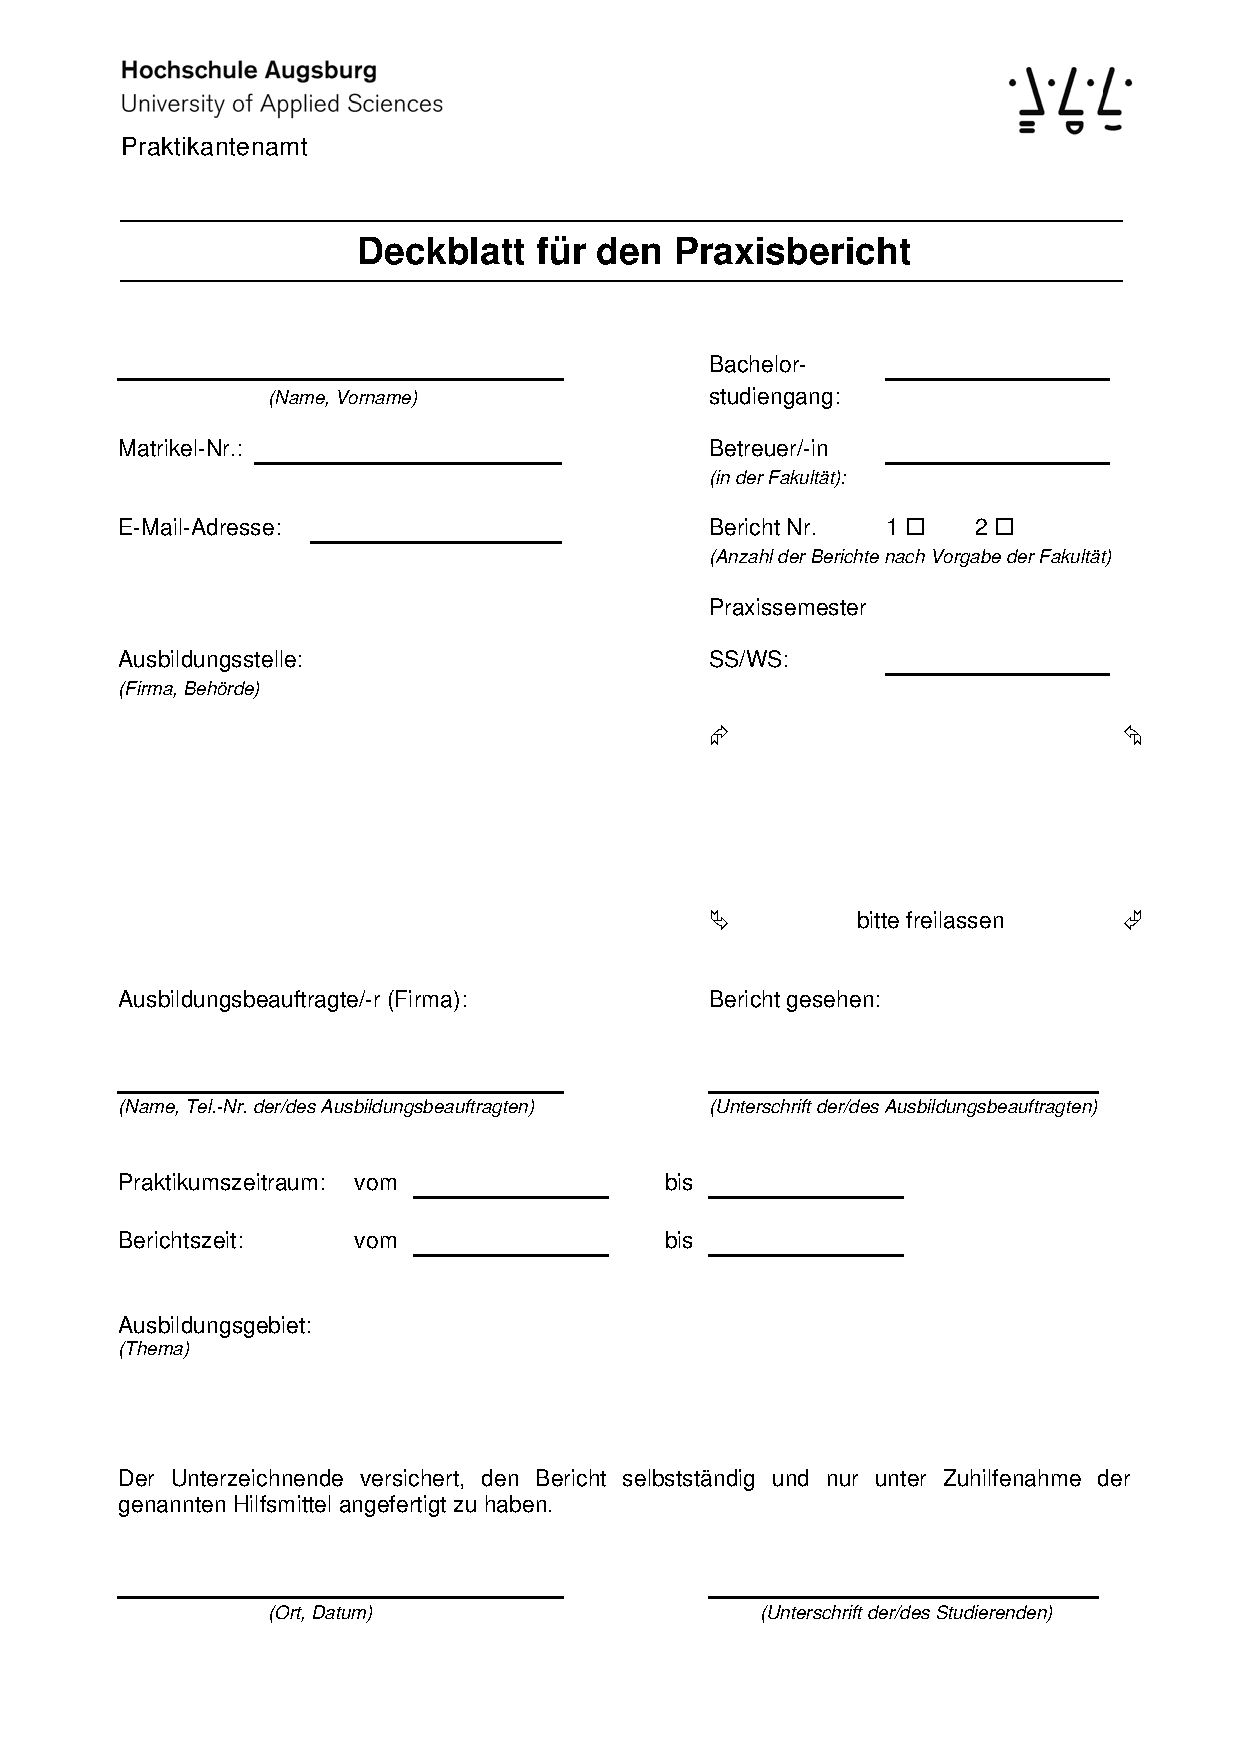
\includegraphics[width=0.93\paperwidth]{figures/deckblatt_prax_bac}
	\label{fig:deckblatt_prax_bac}
\end{figure}
  %<-- Nach Vorgabe der HS Augsburg

	%%% Deckblatt - Hochschule Augsburg
%%%Deckblatt

\textblockorigin{20mm}{30mm}

\thispagestyle{empty}\null
%%%%Logo - Hochschule Augsburg - Informatik
\begin{textblock}{10}(8.0,1.1)
\begin{figure}[h]
	\centering
		
\includegraphics[width=0.45\textwidth]{logos/hsa_informatik_logo_lq.pdf}
\end{figure}

\end{textblock}

%%% Text unter Logo
\begin{textblock}{15}(12.43,2.1)
	\LARGE
	\textsf{
		\textbf{\textcolor[rgb]{1,0.41,0.13}{\\
			\begin{flushleft}
				Fakult�t f�r\\
				Informatik\\
			\end{flushleft}
			}
		}
	}
\end{textblock}

%%%%Textbox links - Informationen
\begin{textblock}{15}(2,1.4)
	%\LARGE
	\begin{flushleft}
		\begin{spacing} {1.2}
			\huge	
				\textbf{Methoden der KI\\}
				\vspace{30pt}
				\textcolor[rgb]{1,0.41,0.13}{\\
				\textbf{Portfoliopr�fung}}\\
				\vspace{60pt}
			\LARGE
				Studienrichtung\\
				Technische Informatik\\
				\vspace{40pt}
				
				Muhammad Aman Bin Ahmad Tifli\\
				\vspace{30pt}		
				Matrikelnummer: 2042550\\
				% \vspace{30pt}		
				% Ausbildungsstelle: KUKA Deutschland AG\\
				\vspace{60pt}		
			\LARGE
				Pr\"ufer: Prof. Dr. Thomas Rist\\
				\vspace{10pt}		
				Abgabedatum: xx.xx.2021\\
			\end{spacing}
		\end{flushleft}
		
\end{textblock}



%%%%Textbox rechts - Hochschule
\begin{textblock}{5}(12.45,9.0)
	\scriptsize
	\textcolor[rgb]{1,0,0}{\\
		\begin{flushleft}
			\begin{spacing} {1.3}
				Hochschule f\"ur angewandte\\
				Wissenschaften Augsburg\\
				\vspace{4pt}
				An der Hochschule 1\\
				D-86161 Augsburg\\
				\vspace{4pt}
				Telefon +49 821 55 86-0\\
				Fax +49 821 55 86-3222\\
				www.hs-augsburg.de\\
				info(at)hs-augsburg-de
			\end{spacing}
		\end{flushleft}
		}
\end{textblock}


%%%%Textbox rechts unten - Fakult?t und Autor
\begin{textblock}{5}(12.45,11.5)
	\scriptsize
		\begin{flushleft}
			\begin{spacing} {1.3}
				Fakult\"at f\"ur Informatik\\
				Telefon +49 821 55 86-3450\\
				Fax \hspace{10pt} +49 821 55 86-3499\\
				\vspace{6pt}
				Verfasser der Diplomarbeit\\
				Max Mustermann\\
				Beispielstra?e 31\\
				86150 Augsburg\\
				Telefon +49 821 55 86-3450\\
				max@hs-augsburg.de\\
			\end{spacing}
		\end{flushleft}
	\end{textblock}
\pagebreak  %<-- Nach Vorgabe der HS Augsburg
	%
	%%%% Innere Titelseite 
 	%\include{titelseite} %<-- Vorgabe Prüfer oder frei wählbar
	%
	%%%%Optional - Falls von der Firma gefordert
	%\include{sperrvermerk}
	%
	%%%%Pflicht
 	%\include{erklaerung}
	%
	%%% Leere Seite bei zweiseitigem Druck
	%\ifnotonesideelse{\blankpage}{}
	%\include{kurzfassung}
	%%% Leere Seite bei zweiseitigem Druck
	%\ifnotonesideelse{\blankpage}{}
%}



%
%% ++++++++++++++++++++++++++++++++++++++++++
%% Verzeichnisse
%% ++++++++++++++++++++++++++++++++++++++++++
\pagenumbering{roman}
\ifnotdraft{
\tableofcontents
% Leere Seite bei zweiseitigem Druck
%\ifnotonesideelse{\blankpage}{}
%\listoffigures
%% Leere Seite bei zweiseitigem Druck
%\ifnotonesideelse{\blankpage}{}
%\listoftables
%% Leere Seite bei zweiseitigem Druck
%\ifnotonesideelse{\blankpage}{}
}
%% ++++++++++++++++++++++++++++++++++++++++++
%% Hauptteil
%% ++++++++++++++++++++++++++++++++++++++++++
\graphicspath{{figures/}}
\pagenumbering{arabic}

%%% Ab hier eigene Kapitel einfügen
%%% Kapitel sind analog zur Wordvorlage zu wählen

\chapter{Introduction}
\chapter{Formulierung von Problemen und Lösungen in der Symbolischen Informationsverarbeitung}
\chapter{Probleml�sung als Suchaufgabe}

\section{Wegsuche ohne Karte}

``Wegsuche ohne Karte'' bedeutet Wegfindung in einer unbekannten Umgebung ohne eine Karte, die den Agenten leitet.

Beispiel: \textbf{Roboter R} befindet sich in einem unbekannten Gebiet und muss sich zu einem Zielobjekt bewegen. Dies kann durch Anwendung eines \textbf{Bug-Algorithmus} gel�st werden, der voraussetzt, dass der Roboter mit Sensoren ausgestattet ist, um Hindernisse und das \textbf{Zielobjekt S} zu erkennen.

\subsection{Bug Algorithmen Beispiel}
\label{bug-algo-1}
Ein Beispiel f�r einen Bug-Algorithmus ist wie folgt:
\begin{enumerate}
    \item Wenn das \textbf{Zielobjekt S} in Sichtweite ist, fahrt \textbf{Roboter R} direkt darauf zu
    \item Wenn \textbf{S} nicht in Sicht ist, aber stattdessen ein Hindernis vorhanden ist, bewegt sich \textbf{R} gem�� einer bestimmten Regel um das Hindernis herum (z. B. im Uhrzeigersinn).
    \item \textbf{R} scannt erneut nach dem Objekt \textbf{S} und wiederholt die Schritte 1 und 2, bis das Ziel erreicht ist.
\end{enumerate}

\begin{figure}[H]
    \centering
    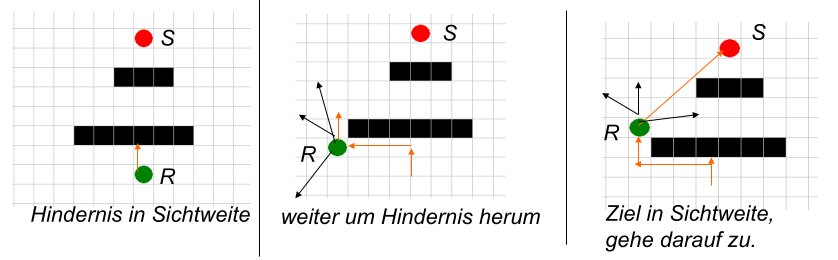
\includegraphics[width=\textwidth]{figures/kap3/bug-algo-1.png}
    \caption{Beispiel von Bug-Algorithmus Verfahren}
    \label{fig:bug-algo}
\end{figure}

\subsection{Problem mit dem Bug-Algorithmus}

In bestimmten Situationen (z.B siehe Abb. \ref{fig:bug-algo-prob}) ist der Roboter mit dem Ansatz in Abschnitt~\ref{bug-algo-1} nicht in der Lage, das Ziel zu finden.

\begin{figure}[H]
    \centering
    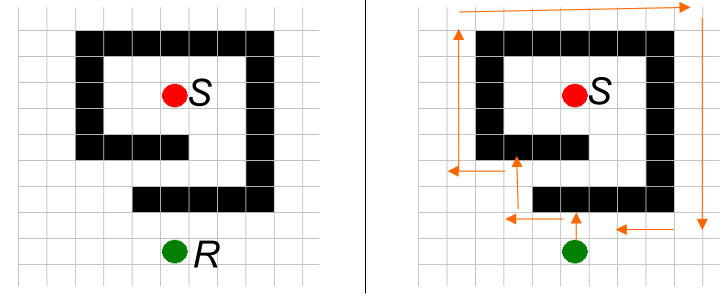
\includegraphics[width=0.8\textwidth]{figures/kap3/bug-algo-1-problem.png}
    \caption{Der Roboter kann das Ziel nicht sehen}
    \label{fig:bug-algo-prob}
\end{figure}

Der Algorithmus muss verbessert werden, z. B. durch Bewegen gegen den Uhrzeigersinn, um eine Bewegung in einem kontinuierlichen Kreis zu vermeiden.

\begin{figure}[H]
    \centering
    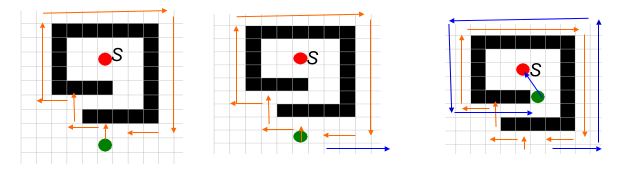
\includegraphics[width=\textwidth]{figures/kap3/bug-algo-1-fix.png}
    \caption{Gegen den Uhrzeigersinn bewegen, um das Ziel zu erreichen}
    \label{fig:bug-algo-fix}
\end{figure}

\section{Repr�sentation von Suchr�umen}

\subsection{Suchraum als Karte}

Ein Suchraum wird normalerweise als grafische Karte dargestellt. Diese Karten k�nnen als Wegenetz oder als Gitter mit benachbarten Zellen dargestellt werden, wie in Abbildung \ref{fig:graph-examples} gezeigt.

\begin{figure}[H]
    \centering
    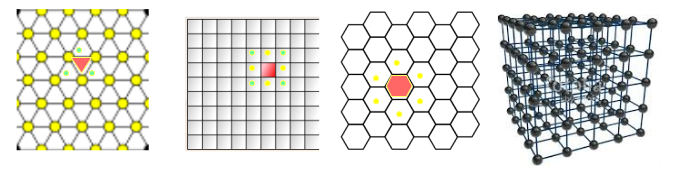
\includegraphics[width=\textwidth]{figures/kap3/graph-examples.png}
    \caption{Beispiele von Gittermustern}
    \label{fig:graph-examples}
\end{figure}

Je nach verwendetem Gittermuster werden unterschiedliche Suchgraphen basierend auf der Anzahl der Nachbarn jeder Zelle im Gitter gebildet. Zum Beispiel: Eine dreieckige Zelle hat sechs Nachbarn, eine quadratische Zelle hat 4 (oder 8, wenn Diagonalen erlaubt sind) und eine sechseckige Zelle hat 6.

\section{Wegsuche als systemstisches Ablaufen von Graphen}

Bei der Wegfindung mit Hilfe eines Graphen m�ssen ein \textbf{Startknoten} und eine \textbf{Funktion zum Testen}, ob der Zielknoten erreicht wurde, definiert werden. Mit Hilfe des Startknotens und dieser Funktion kann eine Folge von Knoten gefunden werden, die die Testfunktion erf�llen k�nnen. Wichtig ist, dass die f�r die Sequenz ausgew�hlten Knoten \textbf{benachbarte Knoten sind, die durch Kanten verbunden} sind.

\subsection{Expliziter Graphen und sukzessive Expansion}

Es ist wichtig, zwischen einem expliziten Graphen und einem ``gedachten'' Graphen als Repr�sentation eines Suchraums f�r L�sungen zu unterscheiden.

\paragraph{Expliziter Graphen}

Eine explizite Darstellung der Knoten und Kanten ist verf�gbar (z.B Adjazentmatrix). Dies ist nur f�r kleinere Knotenmengen praktikabel und die meisten Probleme erfordern keine vollst�ndige Repr�sentation des Suchgraphen.

\paragraph{Sukzessive Expansion}

Diagramm ist verf�gbar, aber nicht vollst�ndig explizit. Der Suchprozess erfolgt durch Knotenerweiterung, indem Knoten f�r Knoten vorgegangen wird.

\subsection{Generelle Wegfindungsstrategie}

Zyklen und Mehrfachbesuche sind zu vermeiden, da sie den Suchbaum exponentiell wachsen lassen k�nnen. Generell sollte man keinen bereits benutzten Weg nochmal gehen, keine Wege mit Zyklen kreieren, einen bereits besuchten oder ausgebauten Zustand nicht nochmal besuchen oder erzeugen.

\subsection{Generelle Bewertung von S uchverfahren} 

Bewertungskriterien eines Pfadfindungsprozesses sind wie folgt:

\paragraph{Korrektheit}

Es ist wichtig, dass die Wegfindungsl�sung tats�chlich eine L�sung des Problems ist.

\paragraph{Vollst�ndigkeit}

Existiert eine L�sung, terminiert der Algorithmus nach endlicher Zeit und generiert eine L�sung.

\paragraph{Optimalit�t}

Die optimalste L�sung wird gefunden, wenn mehrere m�glich sind.

\paragraph{Zeitkomplexit�t}

Die Zeit, die im worst-case/average-case ben�tigt wird, um eine optimale L�sung zu finden.

\paragraph{Speicherkomplexit�t}

Wie viel Speicher, die im worst-case/average-case ben�tigt wird.



\section{Arten von Suchverfahren}

Es gibt viele M�glichkeiten, eine Wegfindungssuche durchzuf�hren. Diese n�chsten Abschnitte werden darauf eingehen.

\subsection{Breitensuche in expliziten Graphen}
\label{section:breitensuche}
Breitensuche ist auf Englisch ``breadth first search''. F�r diesen Algorithmus werden f�r jeden Knoten zus�tzliche Daten ben�tigt: \textbf{noch nicht gesucht} (wei� dargestellt), \textbf{entdeckt, aber noch nicht verarbeitet } (grau dargestellt), \textbf{verarbeitet} (schwarz dargestellt). 

\paragraph{�berblick �ber den Ablauf:}

\begin{enumerate}
    \item W�hle einen Startknoten aus dem Graphen und legen Sie diesen in die Warteschlange, Q. Alle Knoten in Q sind grau markiert.
    \item Solange es Elemente in Q gibt, markiere alle Nachbarn der Elemente grau und f�ge diese der Warteschlange Q hinzu. 
    \item Nachdem alle Nachfolger eines Knotens grau markiert wurden, markiere den Knoten schwarz und entferne ihn aus der Warteschlange. Pr�fen Sie, w�hrend Sie die Nachfolgerknoten grau markieren, ob der zu markierende Knoten der Zielknoten ist.s
    \item Wiederhole Schritt 2 und Schritt 3, bis die Warteschlange Q leer ist.
\end{enumerate}

\paragraph{Komplexit�tsbetrachtung}

Speicherbedarf und Zeitbedarf sind exponentiell. Dies f�hrt dazu, dass gro�e Graphen unl�sbar sind und sogar relativ kleine Graphen zu lange brauchen, um praktikabel zu sein (z.B Graphen Tiefe 12 brauch 35 Jahre Rechenzeit).

\subsection{Uniforme Kostensuche}

Bei diesem Suchalgorithmus wird die Breitensuche so ver�ndert, dass auch die \textbf{Kosten der Nachbarknoten} ber�cksichtigt werden. Da die Kosten zweier benachbarter Knoten normalerweise bereits bekannt sind, kann \textbf{die Warteschlange in einen Heap umstrukturiert werden}, der in \textbf{aufsteigender Reihenfolge der Pfadkosten} sortiert ist. Auf diese Weise wird gehofft, dass der k�rzeste Weg vom Startknoten zum Zielknoten gefunden wird.

\subsection{Modifizierte Uniforme Kostensuche / Dijkstra}

Um eine optimale L�sung f�r ein Wegsucheproblem zu finden, ist es notwendig, alternative Pfade parallel zu konstruieren. Wenn sich diese Pfade am selben Punkt treffen, kann der \textbf{k�rzeste Pfad beibehalten werden}, w�hrend der Rest aus dem Suchbaum entfernt wird, um die k�rzeste Gesamtroute zu finden.

Wenn ein Pfad zum Zielknoten gefunden wird, werden alle \textbf{anderen parallelen Pfade fortgesetzt}, es sei denn, ihre Kosten �bersteigen den bereits gefundenen Pfad. Dies f�hrt zu einer besseren Effizienz bei der Suche nach dem k�rzesten Weg. 

\begin{figure}[H]
    \centering
    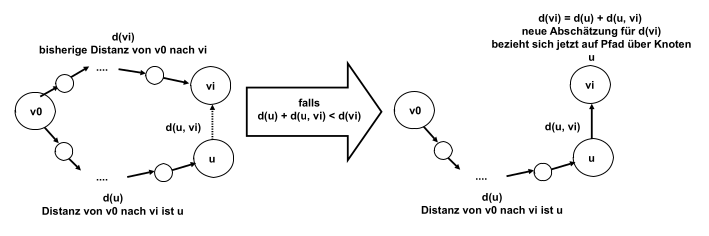
\includegraphics[width=\textwidth]{figures/kap3/dijkstra.png}
    \caption{Dijkstra-Algorithmus Pfadsuche}
    \label{fig:graph-dijkstra}
\end{figure}

Dieser Algorithmus ist in Abbildung \ref{fig:graph-dijkstra} demonstriert. Anhand der Abbildung kann man sehen, wie die beiden Routen von v0 nach vi verglichen werden und die Kosten verglichen werden, um nur die k�rzere Route beizubehalten.

\subsection{Ablauf eines Graphen mit Tiefensuche}

Im Gegensatz zur Traversierung mit Breitensuche verl�uft die Traversierung mit Tiefensuche auf m�glichst langen Wegen und f�hrt die Wei�-Grau-Schwarz-Markierung (siehe Abschnitt \ref{section:breitensuche}) durch. Dieser Algorithmus wird normalerweise rekursiv implementiert.

\paragraph{Ablauf von Tiefensuche}

\begin{enumerate}
    \item W�hle einen Startknoten \( v_s \). Markiere den Knoten als grau ein.
    \item F�r jeden Nachbarknoten \( v_k \) von \( v_s \), der wei� markiert ist, f�hre folgendes durch:
    \begin{enumerate}
        \item F�ge \( v_k \) zum Stack hinzu
        \item Markiere \( v_k \) als grau
        \item Falls \( v_k \) Nachbarn hat, f�hre Schritt (2) rekursiv aus
        \item Wenn \( v_k \) keine Nachbarn hat oder seine Nachbarn schwarz markiert sind, markiere \( v_k \) schwarz und entferne \( v_k \) vom Stack
    \end{enumerate}
    \item Der Algorithmus endet, sobald der Stack leer ist.
\end{enumerate}

\paragraph{Komplexit�tsbetrachtung}

Nur benachbarte Knoten des aktuellen Suchpfads werden auf dem Stack gespeichert. Dies bedeutet viel weniger Knotenerweiterungen im Vergleich zur Breitensuche, was zu weniger Speicherverbrauch f�hrt. Die Zeitkomplexit�t ist jedoch ebenso wie die Brreitensuche exponentiell.

\subsection{Tiefensuche und Backtracking-Algorithmen}

In realen Anwendungen beinhaltet eine L�sung die Verwendung vieler verschiedener Komponenten. Die endg�ltige L�sung verwendet daher normalerweise viele Teill�sungen, die m�glicherweise nicht richtig erweitert werden k�nnen (z.B: erreicht die Teill�sung eine Sackgasse). In diesen F�llen muss die Teill�sung durch eine weniger komplexe L�sung ersetzt werden.

\paragraph{Genereller Ablauf von einem Backtracking-Algorithmus}

Gegeben sind ein Array ``SolutionComponents'', das alle Werte der endg�ltigen L�sung enth�lt, und die Funktionen ``FirstTrialValue()'', ``NextTrialValue()'' und ``CheckValid()''.

\begin{enumerate}
    \item Der ersten Komponente wird der erste Versuchswert gegeben:\\~\\
    \lstinline{SolutionComponents[0] = FirstTrialValue(0)}~\\
    \item Die G�ltigkeit der L�sung wird �berpr�ft:\\~\\
    \lstinline{CheckValid(SolutionComponents)}~\\
    \item Wenn die bisherige L�sung g�ltig ist, fahren Sie mit dem n�chsten Wert fort (i = 1, 2, 3...) und �berpr�fe den Wert erneut\\~\\
    \lstinline{SolutionComponents[i] = FirstTrialValue(i)}~\\
    \lstinline{CheckValid(SolutionComponents)}~\\
    \item Wenn der CheckValid-Funktion an einem bestimmten Punkt false zur�ckgibt, versuche es mit den n�chsten Werten. Wenn alle Werte ebenfalls falsch zur�ckgeben, f�hre ein Backtracking durch, indem Sie i um i reduzieren und den n�chsten Wert f�r dieses i versuchen.Erh�hen Sie dann i wieder um 1 und probieren Sie alle Werte aus.
    \item Schritt 4 wird so oft wie n�tig wiederholt. F�r den Fall, dass i null erreicht und es keine Versuchswerte mehr f�r i = 0 gibt, gibt es keine m�gliche L�sung.
\end{enumerate}

\subsection{Limitierte Tiefensuche}

Es ist m�glich, die Nachteile der Tiefensuche zu vermeiden, indem man eine maximale Tiefe des Pfades einstellt. Das macht die Suche vollst�dnig aber nicht immer optimal. Um diese Idee zu erweitern, kann eine iterative Tiefensuche versucht werden. 

\subsection{Iterative Tiefensuche}

Bei dieser Methode wird die Tiefe mit jeder Iteration erh�ht, um sicherzugehen, dass eine L�sung gefunden wird.

\subsection{Bidirektionale Suche}

Anstatt nur vom Startknoten aus zu beginnen, f�hren Sie eine Suche vom Start- und vom Zielknoten aus durch. Wenn sich die beiden Verfahren in der Mitte treffen, ist eine L�sung gefunden.

\section{KI-Suchverfahren}

Es gibt zwei Klassen von Suchverfahren: \textbf{blinde Suchverfahren} und \textbf{KI-Suchverfahren}. Blinde Suchverfahren sind auf einem bestimmten Schema basiert, das unabh�ngig von dem jeweiligen Problem ist. Einige Beispiele hierf�r sind die in den vorangegangenen Kapiteln behandelten Verfahren wie Breitensuche, Tiefensuche, Biridketionale Suche usw. 

KI-Suchverfahren hingegen nutzen problemspezifisches Vorwissen zur Eingrenzung des Suchraums. Es handelt sich um informierte heuristische Suchverfarhen.

\textbf{Blinde Suchverfahren} erfordern, dass eine L�sung durch systematische und ersch�pfende Suche in einem Suchgraphen gefunden wird, was ineffizient und kein problemspezifisches Wissen nutzt.

\textbf{Informierte Suchprozesse} hingegen nutzen problemspezifische Eigenschaften, um die Effizienz der Knotenexpansion zu verbessern.

\subsection{Greedy Search}
\label{section:greedy-search}
Die Greedy-Suche ist eine modifizierte Breitensuche (siehe Abschnitt \ref{section:breitensuche}), bei der nur die Knoten mit den geringsten Kosten in die Warteschlange aufgenommen werden. 

\paragraph{Ablauf von Greedy Search}

Wenn die Kosten des aktuellen Knotens zum Zielknoten unbekannt sind, \textbf{m�ssen diese Kosten gesch�tzt werden}, und dann wird der Nachbar mit den geringsten Kosten ausgew�hlt. Die Funktion, die diese Kosten sch�tzt, wird \textbf{heuristische Funktion} genannt.

Der Unterschied zwischen Greedy Search und Uniform Cost Search (siehe Abschnitt \ref{section:uniform-cost-search}) besteht darin, dass bei der Greedy Search \textbf{die Kosten von einem Knoten zum Zielknoten} berechnet werden und nicht von einem Knoten zum anderen.

\paragraph{Eigenschaften von Greedy Search}

Greedy Search bietet tendenziell schnelle L�sungen, die oft, aber nicht immer, der optimale Weg sind. 

Greedy Search ist �hnlich wie die Tiefensuche mit Backtracking, nicht vollst�ndig, und erfordert eine gute Heuristik f�r eine bessere G�te des Verfahrens.

\subsection{Der A* Algorithmus}

Der A*-Algorithmus ist ein neuer Ansatz, der auf Greedy Search (Abbschnitt~\ref{section:greedy-search}) und dem Dijkstra-Algorithmus~(Abbschnitt~\ref{section:dijkstra}) aufbaut. A* arbeitet basierend auf der Funktion:

\[f(n) = g(n) + h(n)\]

Wobie \(f(n)\) die gesch�tzten Kosten der billigsten L�sung ist, \(g(n)\) die Kosten f�r die Bewegung von der Ausgangszelle zur aktuellen Zelle, und \(h(n)\) die gesch�tzten Kosten f�r die Bewegung von der aktuellen Zelle zur Zielzelle. Mit der Funktion \(f(n)\) werden die Kosten berechnet, und der Rest des Algorithmus l�uft wie bei Greedy Serach ab.

\subsection{Pfadplannung mit A*}

\subsection{Pfadplannung in Computerspielen}



\section{Vertiefungsprojekt: A*-Pfadfindung}

Um besser zu verstehen, wie die A*-Pfadfindung funktioniert (und um etwas Spa� beim Programmieren zu haben), wurde der Algorithmus in Java implementiert. Diese Umsetzung basiert auf einem Online-Artikel von Baeldung\cite{a-star-online}. Die Struktur des Gesamtprojekts und seine Durchf�hrung werden in Kapitel \ref{section:vertiefungs-projekt} erl�utert. 

\begin{figure}[H]
    \centering
    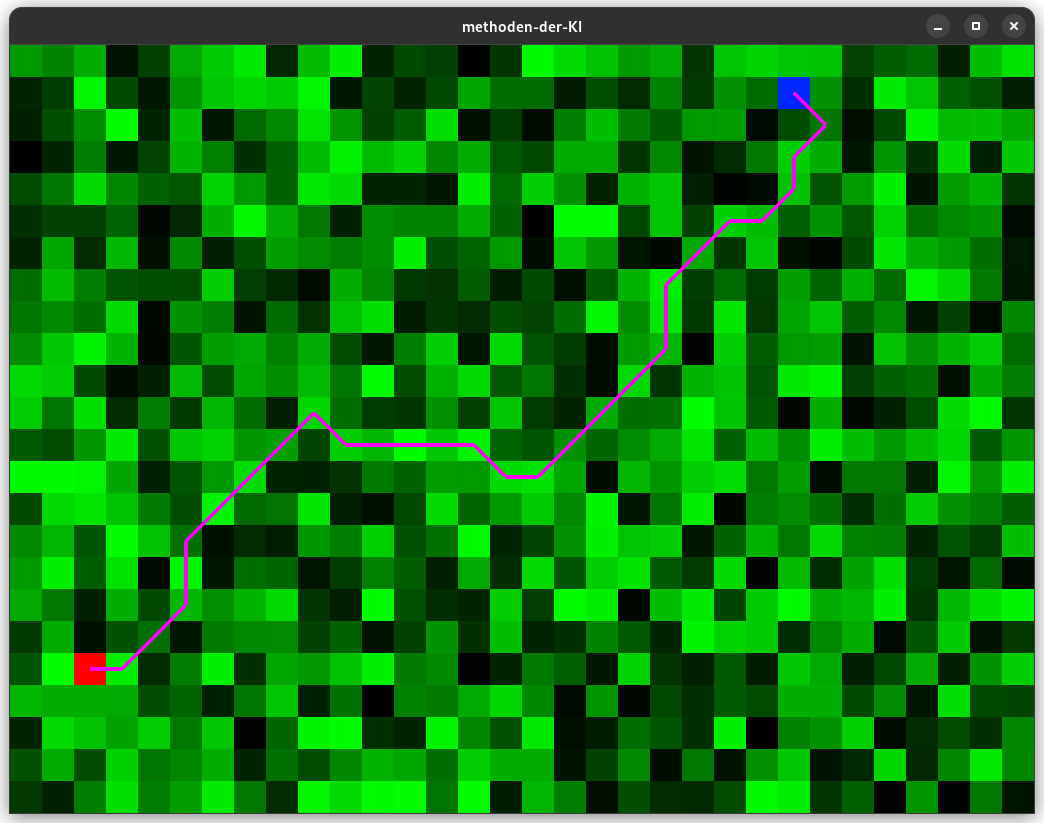
\includegraphics[width=\textwidth]{figures/kap3/a-star-impl.png}
    \caption{Der A*-Pfadfindungs-Screen}
    \label{fig:impl-a-star-pathfinding}
\end{figure}

Bei der Umsetzung wird ein zuf�lliges Terrain in Form von gr�nen Quadraten erzeugt. Je dunkler das Quadrat ist, desto h�her sind die Kosten f�r die Durchquerung des Quadrats. Die Wegfindung beginnt beim roten Quadrat und endet beim blauen Quadrat.

Auf dem A*-Pfadfindungs-Screen des Programms sind die Tastensteuerungen wie folgt:
\begin{itemize}
    \item \textbf{Leertaste:} Erzeugt neues zuf�lliges Terrain und zuf�llige Start- und Endpositionen (Erzeugt eine neue Pfadfindungsaufgabe). 
    \item \textbf{Eingabetaste:} Startet den A*-Pfadfindungsprozess. Der gefundene Pfad wird auf dem SCreen in Form einer hellvioletten Linie angezeigt.
    \item \textbf{Escape-Taste:} Geht zur�ck zum Start-Screen.
\end{itemize}

Es gibt einen Bug im Programm, wodurch manchmal ein Pfad nicht gefunden werden konnte, wenn sich das Ziel am Rand befindet. In diesem Fall wird oben links im Fenster die Meldung ``No traversable route found'' angezeigt.

Der relevante Code f�r das Programm befindet sich in den folgenden Packages (Implementierungscode befindet sich im ``core'' Verzeichnis):
\begin{itemize}
    \item \textbf{de.augsburg.hs.methoden.ki.screens.astar:} Der Code f�r den A-Star-Pathfinding-Screen. Hier kommt der gesamte Code zusammen.
    \item \textbf{de.augsburg.hs.methoden.ki.algorithms.astar:} Allgemeine Implementierung des A*-Wegfindungsalgorithmus.
    \item \textbf{de.augsburg.hs.methoden.ki.algorithms.astar.implementation:} Implementierung des allgemeinen Algorithmus f�r dieses Programm.
    \item \textbf{de.augsburg.hs.methoden.ki.actors.astar:} Enth�lt nur die beiden Actors zum Anzeigen der Start- und Zielquadrate.
\end{itemize}
\chapter{Suchverfahren f�r Strategiespiele}

Es gibt viele Arten von Spielen, die eine KI erfordern, um gegen sie zu spielen, z. B. rundenbasierte Strategie- oder Kartenspiele, Strategiespiele mit einem Zufallselement (z. B. W�rfel) und Spiele, die eine strategische Positionierung von Einheiten erfordern.

Im Gegensatz zu normalen Suchproblemen sind Spiele insofern einzigartig, als der Gegner unberechenbar ist und die Rechenleistung normalerweise begrenzt ist.

\section{MiniMax-Algorithmus}

MiniMax ist ein Algorithmus f�r rundenbasierte Nullsummenspiele. Bei diesem Algorithmus \textbf{maximiert} Spieler A seine Gewinnchancen, wobei er davon ausgeht, dass Spieler B versuchen wird, die Gewinnchancen von Spieler A zu \textbf{minimieren}.

\subsection{Ablauf des MiniMax-Algorithmus}

Der Algorithmus l�uft wie folgt ab:

\begin{enumerate}
    \item Erzeuge eines Suchbaums, wobei die Wurzel die Startposition des Spiels ist und das Ende des Baums die m�glichen Endzust�nde des Spiels darstellt.
    \item Berechne die Gewinnchancen f�r Spieler A f�r jeden Zweig von den Endzust�nden zur�ck zum Ursprung berechnet.
    \item F�r jede Ebene im Suchbaum berechne der Wert f�r die Gewinnchancen von A eines Knotens aus den Werten seiner Nachfolgeknoten. Falls Spieler A am Zug ist, dann ist der Knotenwert der Maximum der Nachfolger, und falls Spieler B am Zug ist, dann ist der Knotenwert der Minimum der Nachfolger.
    \item Nachdem alle Knoten berechnet wurden, w�hlt Spieler A den Weg, der ihm am meisten n�tzt.
\end{enumerate}

Dies l�sst sich am besten anhand eines einfachen Spiels namens ``Nimm'' demonstrieren (siehe Abb. \ref{fig:minmax-nimm-example}). In diesem Spiel gibt es n Objekte. Die Spieler entfernen abwechselnd 1, 2 oder 3 der Objekte. Der Spieler, der das letzte Objekt nimmt, verliert.

\begin{figure}[H]
    \centering
    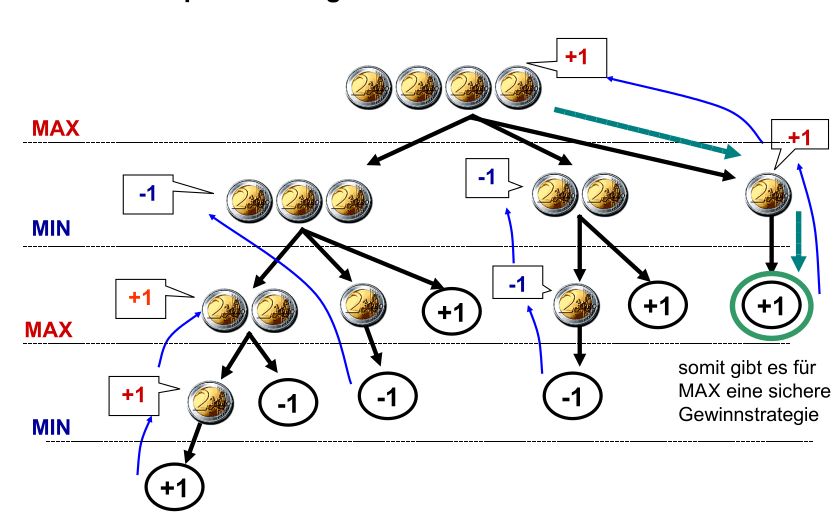
\includegraphics[width=0.8\textwidth]{figures/kap4/minmax-nimm.png}
    \caption{Bottom-up Bewertung der Knoten aus der Sicht von MAX}
    \label{fig:minmax-nimm-example}
\end{figure}

\subsection{Eigenschaften des MiniMax-Algorithmus}

Der Algorithmus ist vollst�ndig, wenn der Suchbaum endlich ist, und ist optimal, wenn gegen einen optimalen Spieler gespielt wird. Der Algorithmus hat ein Zeitbedarf von \(O(b^m)\) miz Suchtiefe \(m\) und Verzweigungsfaktor \(b\) und hat ein Platzbedarf von \(O(b*m)\). 

Dieser Algorithmus kann modifiziert werden, indem man die Tiefe des Baumes begrenzt (nur ein paar Runden vorausschaut) und den Nutzen einer Position mit einer guten Bewertungsfunktion absch�tzt.

\subsection{Verbesserung des MiniMax-Algorithmus durch Pruning}

Pruning, auch bekannt als \(\alpha\beta\)-Search oder \(\alpha\beta\)-Pruning, ist eine Idee, um die Effizienz des Minimax-Algorithmus zu verbessern, indem fr�hzeitig erkannt wird, welchem Zweig des Suchbaums nicht gefolgt werden muss.

Unter der Annahme, dass MIN und MAX jeweils den f�r sie optimalen Weg w�hlen, ist es m�glich fr�hzeitig zu erkennen, welche Verzweigungen des Suchbaums das Ergebnis nicht beeinflussen und daher nicht berechnet werden m�ssen. Unter Verwendung des Nimm-Beispiels k�nnen Pfade geschnitten werden, die ein schlechteres Ergebnis liefern als bereits erkundete Pfade.

\begin{figure}[H]
    \centering
    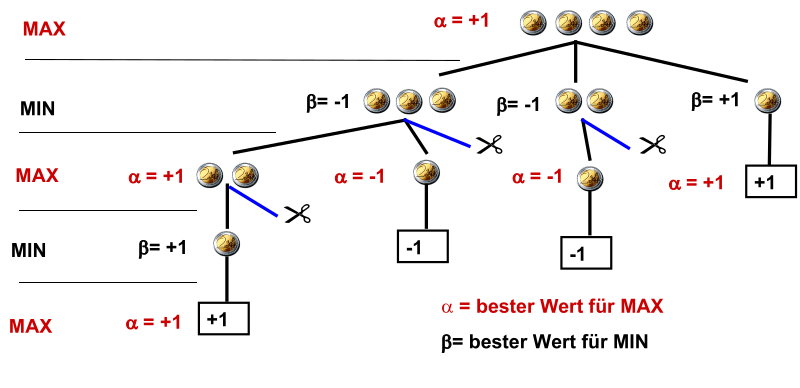
\includegraphics[width=0.8\textwidth]{figures/kap4/minxmax-pruning.png}
    \caption{Beschneiden des MinMax-Nimm-Beispiels}
    \label{fig:minmax-pruning-example}
\end{figure}

\subsection{Komplexit�t von MiniMax-Pruning}

Im schlimmsten Fall, wenn die Knoten in einer ung�nstigen Reihenfolge sind, dann ist es dasselbe wie bei einem normalen MiniMax. Im besten Fall k�nnte man die Mindestanzahl an Positionen berechnen lassen. Dies kann erreicht werden, indem die Reihenfolge der Bewegungen basierend auf der Effizienz der Bewegung neu geordnet wird. Zum Beispiel ist beim Schach das Schlagen einer Figur mit einem Turm oft vorteilhaft und sollte zuerst sequenziert werden.

\subsection{MiniMax in Spielen mit Zuf�lligkeit}

Die Zuf�lligkeit wird unter Verwendung zus�tzlicher Knoten im Suchbaum gehandhabt. F�r die Bewertung erh�lt jeder Zweig der Zufallsknoten den Durchschnitt aller m�glichen Zufallsergebnisse. 

\begin{figure}[H]
    \centering
    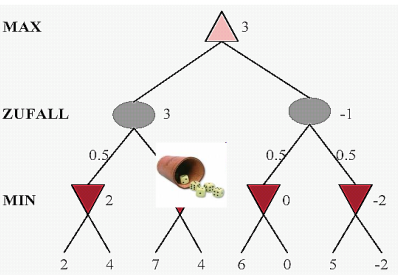
\includegraphics[width=0.6\textwidth]{figures/kap4/minmax-random.png}
    \caption{Zus�tzlicher Zufallknoten mit Mittelwert-Bewertung}
    \label{fig:minmax-random-example}
\end{figure}

\section{Monte Carlo Tree-Search}

In gro�en Suchr�umen wie Schach oder Go ist der MiniMax-Algorithmus weniger geeignet, da zu viele Knoten erweitert werden m�ssten. Die Idee von Mote Carlo Tree Search (MCTS) ist, dass ein Suchbaum wie in MiniMax ebenfalls generiert wird, aber anstatt alle m�glichen Positionen zu erweitern, werden die Z�ge durch zuf�llige Z�ge �ber (sehr) viele Spiele erweitert.

\subsection{Ablauf des MCTS-Algorithmus}

Die folgenden Schritte werden wiederholt durchgef�hrt:-

Die folgenden Schritte werden so lange wiederholt, bis der Alhorithmus zum Abbrechen aufgefordert wird:

\begin{enumerate}
    \item \textbf{Selection}. Max beginnt bei der Wurzel, um einen g�nstigen Zug zu w�hlen. Wenn noch keine Informationen vorliegen, wird ein zuf�lliger Zug gew�hlt.
    \item \textbf{Expansion}. Wenn ein ausgew�hlter untergeordneter Knoten nicht der Endzustand ist, werden alle m�glichen Nachfolger hinzugef�gt und einer ausgew�hlt.
    \item \textbf{Simulation}. Ab dem ausgew�hlten Knotenpunkt wird das Spiel gespielt, bis es mit einem Sieg, einer Niederlage oder einem Remis endet.
    \item \textbf{Backpropagation}. �bertrage die Ergebnisse des Spiels von den Endknoten zur�ck zum Wurzel und aktualisiere die Knoten auf dem Pfad.
\end{enumerate}

Der daraus resultierende Suchbaum sieht in etwa so aus wie in der Abbildung~\ref{fig:monte-carlo-tree-example}.

\begin{figure}[H]
    \centering
    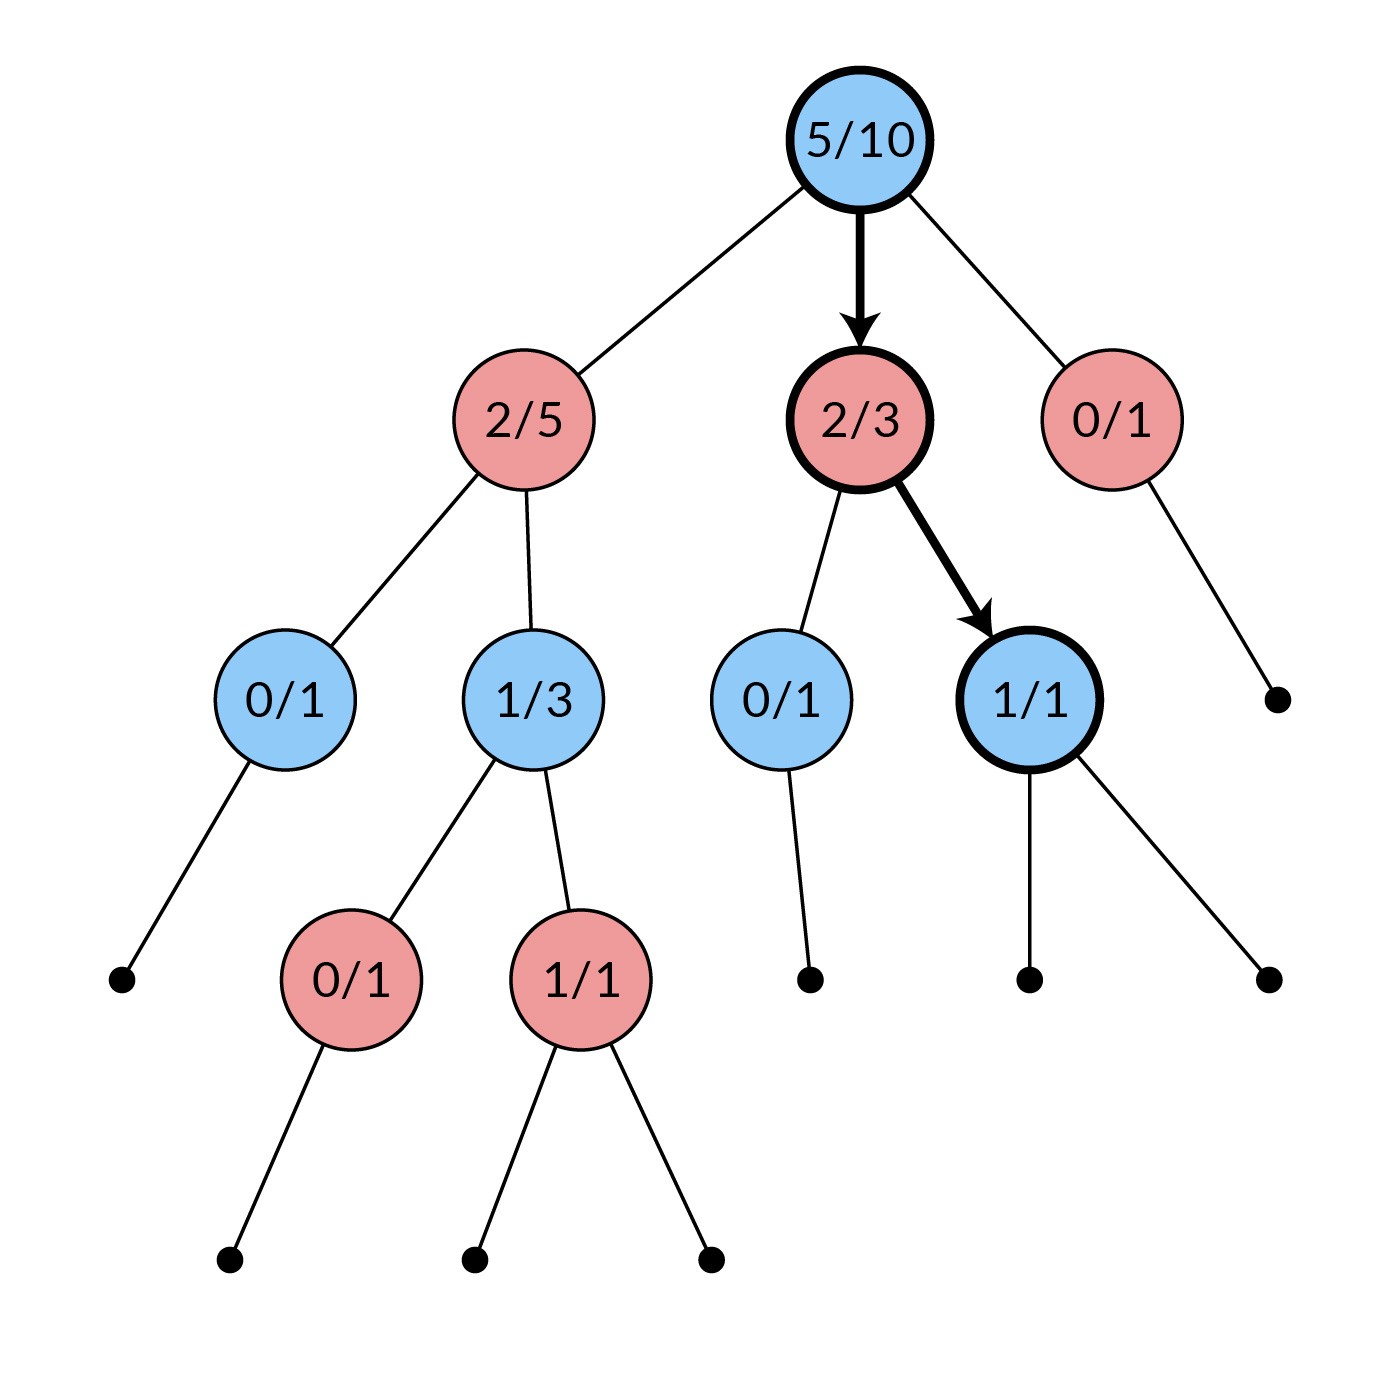
\includegraphics[width=0.65\textwidth]{figures/kap4/monte-carlo-tree-example.jpeg}
    \caption{Beispiel f�r einen Monte-Carlo-Suchbaum}
    \label{fig:monte-carlo-tree-example}
\end{figure}

Jeder Knoten hat einen Wert von \(Siege/Spiele\). Mit diesem Wert kann der beste Knoten basierend auf einem hohen Verh�ltnis von Gewinnen zu gespielten Spielen ausgew�hlt werden.
\chapter{Constraints}

Bei vielen Problemen gibt es Abh�ngigkeiten in den L�sungskomponenten. Es gibt zum Beispiel F�lle, in denen wenn X den Wert A hat dann hat Y den Wert B. Oder wie im Spiel Sudoku kann dieselbe Zahl nicht zweimal in derselben Reihe oder Diagonale vorkommen. Probleme, bei denen Constraints eine Rolle spielen, und wie sie gel�st werden k�nnen, werden in diesem Kapitel behandelt.

\section{L�sen von Constrain-Problemen}

\paragraph{Allgemeines Constraint Solving Problem}

Bei einer gegebenen Menge von Variablen innerhalb eines bestimmten Wertebereichs und einer Menge von Beschr�nkungen erlaubter Kombinationen der Variablenwerte wird nach einer konkreten Anordnung der Variablen gesucht, die alle Beschr�nkungen erf�llen kann.

\paragraph{Constraint Solving Problem als Suche}

Solche Probleme k�nnen als Suchproblem dargestellt werden, wobei:
\begin{itemize}
    \item \textbf{Suchraum:} Menge von Variablen und derren Dom�nen
    \item \textbf{Anfangszustand:} Alle Variables sind noch unbelegt
    \item \textbf{Zielzustand:} alle Variablen belegt und Constraints erf�llt
    \item \textbf{Zieltest:} �berpr�fe, ob alle Variablen die Constraints erf�llen
\end{itemize}

\subsection{Ans�tze z�r L�sung von Constraint Solving Problemen}

\paragraph{Ansatz 1: Generiere und Teste}

Generiere Kombinationen von Werten f�r die Variablen basierend auf ihren Dom�nen und teste, ob die Bedingungen erf�llt sind. Wiederhole so oft wie n�tig.


\begin{table}[H]
    \centering
    \begin{tabular}{|l|l|l|l|}
    \hline
    \(x_1\) & \(x_2\) & \(x_3\) & \textbf{Test} \\ \hline
    1           & 1           & 1           & nein          \\ \hline
    1           & 1           & 2           & nein          \\ \hline
    1           & 2           & 1           & nein          \\ \hline
    1           & 2           & 2           & nein          \\ \hline
    2           & 1           & 1           & nein          \\ \hline
    2           & 1           & 2           & nein          \\ \hline
    2           & 2           & 1           & ja            \\ \hline
    \end{tabular}
    \caption{\label{tab:generate-and-test} Ergebnis des Generierens und Testens}
\end{table}

\paragraph{Ansatz 2: Tiefensuche mit Backtracking}

Die Werte f�r die Variablen werden systematisch generiert, um nicht alle m�glichen Kombinationen generieren zu m�ssen.

\begin{table}[H]
    \centering
    \begin{tabular}{|l|l|l|l|}
    \hline
    \(x_1\) & \(x_2\) & \(x_3\) & \textbf{Test} \\ \hline
    1           & 1           & 1           & nein          \\ \hline
    1           & 1           & 2           & nein          \\ \hline
    1           & 2           & 2           & nein          \\ \hline
    1           & 2           & 1           & nein          \\ \hline
    2           & 2           & 1           & ja            \\ \hline
    \end{tabular}
    \caption{\label{tab:deepsearch-and-backtracking} Ergebnis von Tiefensuche und Backtracking}
\end{table}

Durch den Einsatz von Heuristiken und anwendungsspezifischen Merkmalen kann die L�sung von Constraint-Problemen effizienter gestaltet werden. Unter Verwendung von Constraints kann der Zustandsraum umstrukturiert werden, um die Constraints zum leichteren L�sen des Problems auszunutzen.

\subsection{Optimierung der L�sung von Constraint Problemen}

Die folgenden Optimierungen lassen sich anhand eines konkreten Beispiels besser erkl�ren. Ein Beispiel f�r ein Problem mit Cosntraints ist die Einf�rbung von Staaten in Australien mit drei Farben, so dass benachbarte Staaten niemals dieselbe Farbe haben.

\begin{figure}[H]
    \centering
    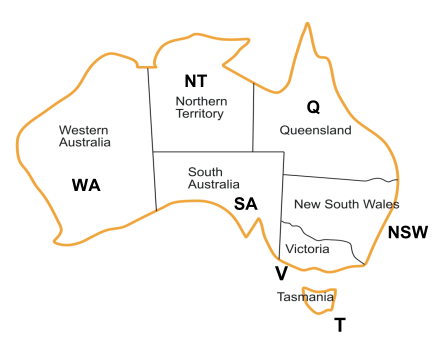
\includegraphics[width=0.6\textwidth]{figures/kap5/australia-map.png}
    \caption{Karte der Staaten von Australien}
    \label{fig:constraints-australia-states}
\end{figure}

\paragraph{Anwendung von Constraint Netzen}

Ein Netz kann erstellt werden, wenn Probleme bin�re Beschr�nkungen haben. Die Variablen sind die Knoten und die Kanten verbinden die Knoten mit Nebenbedingungen.

\begin{figure}[H]
    \centering
    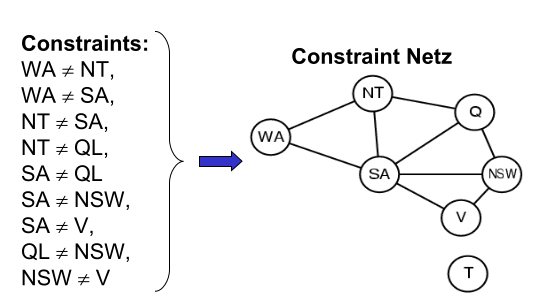
\includegraphics[width=0.6\textwidth]{figures/kap5/australia-constraint-net.png}
    \caption{Constraints-Netz}
    \label{fig:constraint-net-australia}
\end{figure}

Das Constraints Netz kann in Heuristiken verwendet werden, um die Nutzung der Tiefensuche mit Backtracking zu verbessern.

\paragraph{Abalauf von Tiefensuche mit Backtracking zur L�sung von Constraint Problemen}

Mit Hilfe einer \textbf{Degree Heuristik}, bei der mit der Variable begonnen wird, die die meisten Constraints aufweist, kann die Suche optimiert werden. Based on the Constraint Netz in Abb.~\ref{fig:constraint-net-australia}, k�nnen wir sehen, dass SA die meisten Einschr�nkungen hat und die Suche damit beginnen sollte. Danach wird die Suche wie eine typische Tiefensuche (siehe Abschnitt~\ref{section:depth-search-backtracking}) fortgesetzt:-

\begin{enumerate}
    \item In jedem Schritt wird einer Variablen ein Wert zugeordnet.
    \item Wenn die Variable nicht mehr so erweitert werden kann, dass sie den Beschr�nkungen entspricht, wird ein Backtracking durchgef�hrt.
\end{enumerate}

Eine weitere Heuristik, die verwendet werden kann, ist die Minimum-Remaining-Value-Heuristik. 

\section{Vertiefungsprojekt: N-Damen Problem mittels Choco-Solver}

Um besser zu verstehen, wie Constraint-Probleme mit konventionellen Programmiersprachen gel�st werden, wurde das N-Queen-Problem in Java implementiert.

\begin{figure}[H]
    \centering
    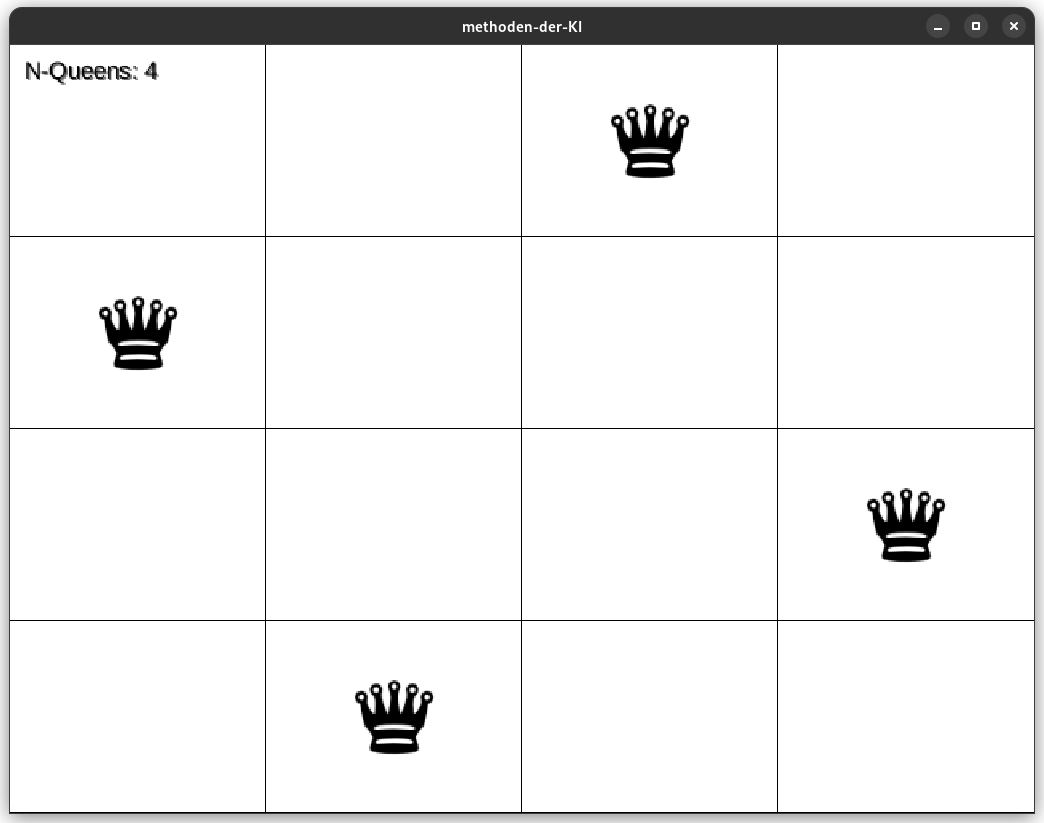
\includegraphics[width=0.8\textwidth]{figures/kap5/n-queens-impl.png}
    \caption{N-Damen Implementierung mit n=4}
    \label{fig:impl-n-damen}
\end{figure}

In diesem Programm wird das n-Damen-Problem f�r n=4 bis 27 unter Verwendung von Constraints gel�st. In diesem Programm w�rde das Dr�cken der Aufw�rts- und Abw�rtspfeiltasten den Wert von N entsprechend erh�hen oder verringern. Das Gitter aktualisiert sich dann selbst, um n x n beizubehalten, und der Choco-Cosntraintssl�ser wird jedes Mal verwendet, wenn sich n �ndert, um eine L�sung zu generieren. Das Programm funktioniert f�r Werte von n von 4 bis 27, aber da die Gr��e des Damenbildes nicht skaliert, ist es schwer zu sehen, wo genau eine Dame nach n=18 platziert wird.

Die Tastensteuerungen wie folgt:
\begin{itemize}
    \item \textbf{Up Arrow Key:} Erh�ht den Wert von N.
    \item \textbf{Down Arrow Key:} Verringert den Wert von N.
    \item \textbf{Escape-Taste:} Geht zur�ck zum Start-Screen.
\end{itemize}

Der relevante Code f�r das Programm befindet sich in den folgenden Packages:
\begin{itemize}
    \item \textbf{de.augsburg.hs.methoden.ki.algorithms.constraints:} Implementierung der Constraints mit Choco-Solver.
    \item \textbf{de.augsburg.hs.methoden.ki.screens.minmax} Klasse f�r den N-Queen-Screen.
    \item \textbf{de.augsburg.hs.methoden.ki.actors.nqueens:} Klassen f�r die Darstellung der Damen.
\end{itemize}

\input{kapitel/5/kap_5.3.tex}

\input{kapitel/5/kap_5.4.tex}
\chapter{Wissensbasierte Systeme}

Wissensbasierte Systeme verwenden wissensbasierte Informationsverarbeitung, um L�sungen f�r Probleme zu berechnen. Diese Art der Informationsverarbeitung ist ein Paradigma, das eine strikte Trennung von Wissen und den zur L�sung des Problems erforderlichen Verarbeitungsmechanismen erfordert.

In einem klassischen System besteht ein Programm aus Programmen und Algorithmen. Ein wissensbasiertes System hingegen besteht aus symbolisch dargestelltem Wissen und Verarbeitungsmechanismen, um dieses Wissen zur Probleml�sung zu nutzen.

\begin{figure}[H]
    \centering
    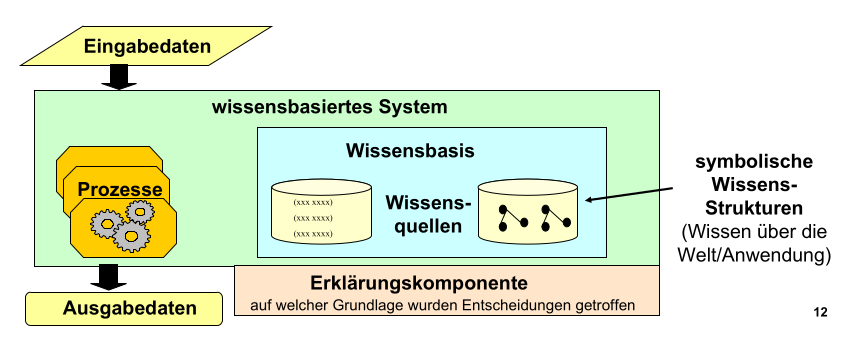
\includegraphics[width=\textwidth]{figures/kap6/anatomie-wbs.png}
    \caption{�berblick �ber ein wissensbasiertes System}
    \label{fig:overview-wbs}
\end{figure}

\section{Wissensdarstellung in wissensbasierten Systemen}

Wissensbasierte Informationsverarbeitung basiert auf der Vorstellung, dass viele Probleme nur l�sbar sind, wenn man Erfahrung mit dem Problem und den L�sungsm�glichkeiten daf�r hat. Dies wirft die Frage auf: Wie stellen wir Wissen so dar, dass es von Computern verstanden und zur Probleml�sung verwendet werden kann?

Wissen wird dabei als Klassen, Kategorien und Konzepte mit Hierarchien, Zusammensetzungen und Klassifikationen dargestellt. Dies ist eine ontologische Erfassung einer Anwendungsdom�ne bekannt. Diese Art der Datenmodellierung l�sst sich am besten mit einer Mindmap vergleichen (siehe Abb.~\ref{fig:mind-map-example}).

\begin{figure}[H]
    \centering
    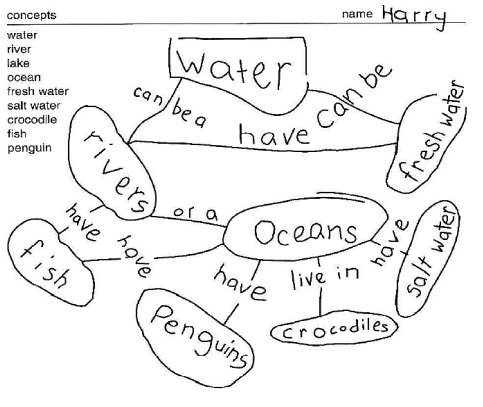
\includegraphics[width=0.52\textwidth]{figures/kap6/mind-map.png}
    \caption{Beispiel einer Mindmap von einem Grundsch�ler}
    \label{fig:mind-map-example}
\end{figure}

Diese Klassen, Kategorien und Konzepte werden letztlich in der Implementierung durch programmtypische Datenstrukturen wie Objekt-Arrays und Pointer abstrahiert (Abb.~\ref{fig:knowledge-darsetllung-ebenen}).

\begin{figure}[H]
    \centering
    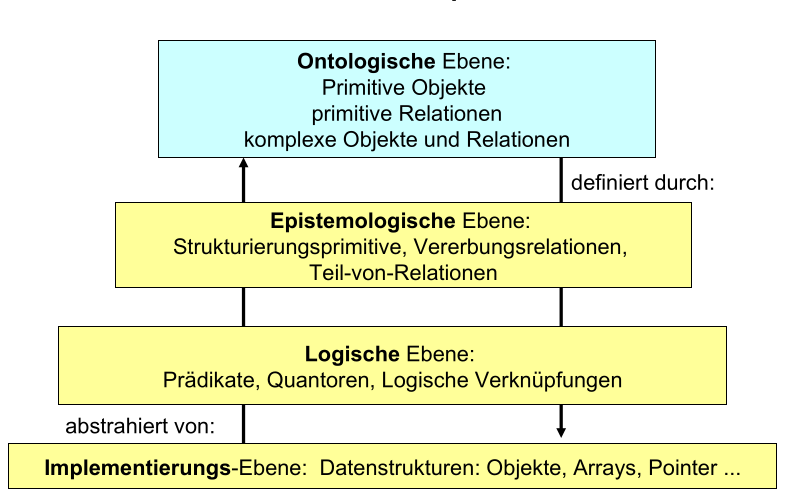
\includegraphics[width=0.8\textwidth]{figures/kap6/ebenen-wissendarstellung.png}
    \caption{Ebenen der Wissensrepr�sentation}
    \label{fig:knowledge-darsetllung-ebenen}
\end{figure}

Es gibt viele M�glichkeiten, Wissen explizit darzustellen. Eine Anwendung kann logikbasierte Ans�tze wie Fakten und Regeln verwenden. Andere k�nnen Rahmen und F�lle oder strukturierte Vererbungsnetze �hnlich objektorientierter Modelle verwenden.

\section{Schnittstelle zur Interaktion mit einem Wissenbassierten System}

Damit ein Benutzer mit einem wissensbasierten System interagieren kann, muss eine Schnittstelle vorhanden sein, die mindestens die folgenden Funktionen ausf�hren kann:

\begin{itemize}
    \item \textbf{Tell(WBS, knowledge-item):} F�ge dem System neues Wissen hinzu. z.B: "Die Welt ist Rund"
    \item \textbf{Ask(WBS, question):} Anfrage stellen. z.B: ist die Welt eine Kugel?
\end{itemize}

Allein durch die Verwendung dieser beiden Funktionen kann ein wissensbasiertes System verwendet werden, um Probleme innerhalb seiner Wissensbasis zu l�sen.

\section{Ans�tze zur Wissensverarbeitung}

Eine wichtige Komponente eines wissensbasierten Systems ist die Inferenzmaschine, die verwendet wird, um unsere Antworten auf Fragen zu finden. Es gibt viele Ans�tze f�r die Implementierung einer solchen Maschine zur Verarbeitung von vorhandenem Wissen.

\paragraph{Prinzip der Wissensabstraktion}

Diese Methode wird als induktive Inferenz bezeichnet: Ableitung allgemeiner Aussagen aus Spezialf�llen. z.B:

\begin{itemize}
    \item Beobachtung: Studenten Hans und Fritz haben ein Laptop
    \item Schlussfolgerung: Alle Studenten haben Laptops
\end{itemize}

\paragraph{Prinzip von Wissen �ber Wissensintegrit�t}

Diese Methode wird als deduktive Inferenz bezeichnet: Durch Erkennung von Regeln und Invarianzen aus formalen Beschreibungen wird explizites Wissen explizit gemacht. z.B:

\begin{itemize}
    \item Beobachtung: Aussage A ist wahr und Aussage B ist wahr.
    \item Schlussfolgerung: Auch die Aussage A oder B ist wahr.
\end{itemize}

\paragraph{Prinzip von Wissen �ber Kausalzusammenh�nge}

Diese Methode wird als abduktive Inferenz bezeichnet: Die Ursachen werden aus Beobachtungen abgeleitet: A ist der Grund daf�r, dass B passiert ist, wenn also B beobachtet wird, ist A passiert. z.B:

\begin{itemize}
    \item Beobachtung: Licht ist an.
    \item Schlussfolgerung: Lichtschalter ist auf Position ``Ein''.
\end{itemize}

\paragraph{Wissen �ber Analogien}

Diese Methode wird als analoge Inferenz bezeichnet: Neue Erkenntnisse werden aus bereits bekannten abgeleitet. z.B:

\begin{itemize}
    \item Beobachtung: durch ein dickes Rohr kann viel Wasser flie�en.
    \item Schlussfolgerung: durch ein dickes Kabel kann viel Strom flie�en.
\end{itemize}

\paragraph{Prinzip der Verwendung von empirischem Wissen}

Diese Methode wird als probabilistische Inferenz bezeichnet: Schlussfolgerung, dass eine Wirkung eintritt, basierend auf der Wahrscheinlichkeit, dass sie aufgrund der Situation eintritt. z.B:

\begin{itemize}
    \item Wenn 100 Personen im Raum sind, kann man davon ausgehen, dass mindestens zwei von ihnen denselben Geburtstag haben.
\end{itemize}

\paragraph{Prinzip der Verwendung von unscharfem Wissen}

Diese Methode wird als Fuzzy-Inferenz bezeichnet: Schlussfolgerungen auf der Grundlage der Wahrscheinlichkeit, dass ein Objekt zu einer Menge geh�rt. z.B:

\begin{itemize}
    \item Hans ist vierzig Jahre alt. Alte Menschen sind weise.
    \item Zugeh�rigkiet Hans zur Menge der jungen Menschen: 0.6
    \item Zugeh�rigkiet Hans zur Menge der alten Menschen: 0.4
    \item Ask: Ist Hans Weise? Antwort: Na ja, geht so
\end{itemize}

\section{Aufgaben beim Entwurf eines Wissenbassierten Systems}

Es ist es wichtig, von Anfang an herauszufinden, welche Arten von Wissen es zu erwerben gilt und wie diese repr�sentiert und gespeichert werden. Daneben muss auch entschieden werden, welche Inferenzmechanismen verwendet werden sollen.

Dann stellt sich die Frage, wie die Wissensbasis gef�llt werden soll. Dazu gibt es einfache Methoden, z. B. indem man einen Experten dazu bringt, sein Wissen mit einem Texteditor, einem Formular oder einem Mikrofon einzugeben. Es gibt aber auch komplexere Ans�tze wie die Entwicklung einer Schnittstelle zur Umwandlung von Datenbankinhalten in ein Format, das von einem wissensbasierten System verarbeitet werden kann, oder die Extraktion neuen Wissens mit Hilfe k�nstlicher neuronaler Netze. 

\section{Vertiefung: The Bitter Lesson}

In dem kurzen Essay von Richard Sutton, einem kanadischen Informatiker, diskutiert er den seiner Meinung nach gr��ten Fehler der KI-Forschung der letzten 70 Jahre. Er argumentiert, dass die KI-Forschung durch einen zu starken Fokus auf die Verwendung von Ans�tzen des ``menschlichen Wissens'' anstelle der Verwendung von Rechenleistung behindert wurde.

Als Beispiel verwies er auf das Jahr 1997, als Kasparov, Schachweltmeister, von einem Computer besiegt wurde, der Deep Search mit spezieller Hard- und Software verwendete, anstatt das menschliche Verst�ndnis der besonderen Natur des Schachs zu nutzen. Diese Methode wurde von der Mehrheit der Computerschachforscher abgelehnt, die entt�uscht waren, dass das System keine Methoden verwendete, die auf menschlichem Input basierten, um zu gewinnen.

�hnliche Situationen gab es bei der Entwicklung von Computer Go, Spracherkennung und Computer Vision. Dabei kamen zun�chst solche Ans�tze: die Besonderheiten des Spiels bei Go, die Kenntnis von W�rtern und Ph�nomenen f�r die Spracherkennung oder die Suche nach Kanten und Zylindern im Computer Vision. Am Ende wurde all dies jedoch zugunsten neuerer Methoden verworfen, die sich die rohe Rechenleistung zunutze machen, die aufgrund des Mooresschen Gesetzes zur Verf�gung gestellt wurde.

Die bitteren Lehren laut Richard Sutton sind, dass die Leistungsf�higkeit von Allzweckmethoden, die mit zunehmender Rechenleistung weiter skalieren, nicht untersch�tzt werden sollte und dass sich die KI-Forschung darauf konzentrieren sollte, KI-Agenten zu erm�glichen, herauszufinden, wie sie die Au�enwelt verstehen k�nnen. und der KI keine bestimmte Denkweise aufzuzwingen.
\chapter{Regelbasierte Wissensverarbeitung und Expertensysteme}



\section{Aufbau eines regelbasierten Wissensbasierten Systems}

Regelbasierte Systeme basieren auf dem Prinzip eines Produktionssystems zur Termersetzung (Emil Post 1943). Eine �bersicht �ber ein komplettes Produktionssystems ist in Abbildung~\ref{fig:xps-overview} dargestellt.

\begin{figure}[H]
    \centering
    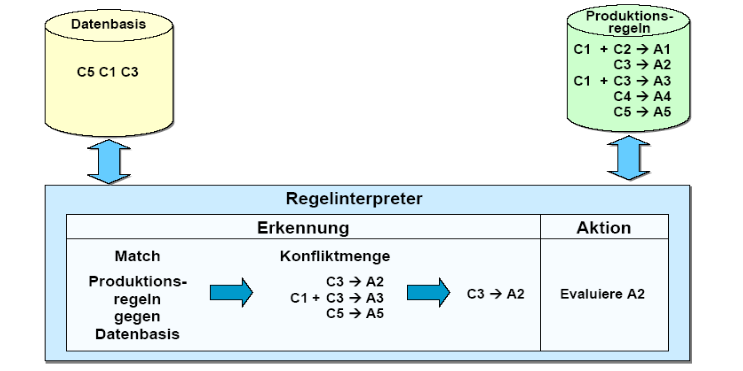
\includegraphics[width=0.9\textwidth]{figures/kap7/overview-xps.png}
    \caption{Produktionssystems zur Termersetzung}
    \label{fig:xps-overview}
\end{figure}

Eine Produktion, auch als ``Regel'' bekannt, besteht aus zwei Teilen (Abb.~\ref{fig:xps-regelstruktur}).

\begin{figure}[H]
    \centering
    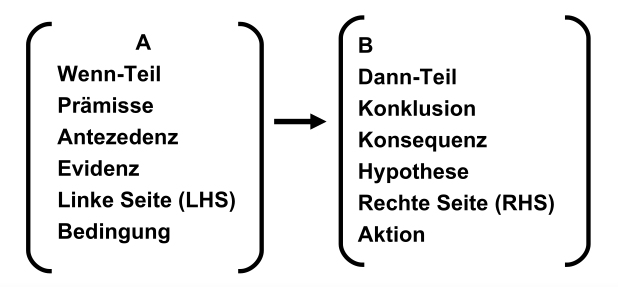
\includegraphics[width=0.8\textwidth]{figures/kap7/production-system-parts.png}
    \caption{Regelstruktur eines regelbasierten Expertensystems}
    \label{fig:xps-regelstruktur}
\end{figure}

Grunds�tzlich basieren die Regeln auf einer Kombination der Teile von A und Teilen von B. Zum Beispiel: Wenn A1 und A2 und An, \textbf{dann} B1 und B2 und Bn und Bm und so weiter. 

Anhand dieser Regeln kann Wissen von Experten gebildet werden. Tats�chlich arbeiten viele Expertensysteme mit einer einfachen Form von IF <Begingung> THEN <Konsequenz>.

\section{Zustandsraumdarstellung eines Wissensverarbeitungsproblems}

Die vier wichtigsten Komponenten f�r so ein System, die man kennen muss, sind Fakten, Regeln und Anfragen. 

\textbf{Fakten} sind Eintr�ge in der Fakten- oder Datenbasis. F�r jedes Problem beginnt das System mit einer Beschreibung des gesamten bekannten Wissens �ber eine Problemstellung. 

\textbf{Regeln} werden verwendet, um einen L�sungsschritt zu erzeugen. Mit Hilfe von Regeln werden neue Fakten ber�cksichtigt und einige fr�here verworfen. Das bedeutet, dass die Faktenbasis durch die Anwendung von Regeln ver�ndert wird.

\textbf{Anfragen}, die als Pr�dikate konstruiert sind, beschreiben die Bedingungen, die ein Problem umgeben. Wenn das Pr�dikat in der Datenbasis gefunden wird (nachdem Fakten einige Regeln durchlaufen haben), ist das Problem gel�st.  

Eine �bersicht �ber die Beziehungen zwischen diesen drei Komponenten ist in Abbildung~\ref{fig:xps-relationships} dargestellt.

\begin{figure}[H]
    \centering
    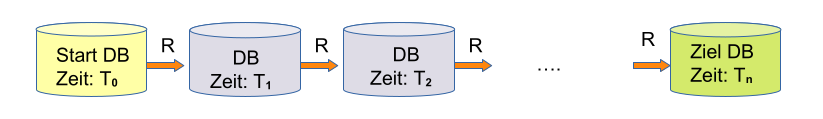
\includegraphics[width=\textwidth]{figures/kap7/state-space-of-xps.png}
    \caption{Beziehung zwischen Fakten, Regeln und Abfragen}
    \label{fig:xps-relationships}
\end{figure}

Dabei ist es wichtig zu beachten, dass der Zustandsraum nicht definiert, wie ein Problem mit den Regeln gel�st werden kann. Hierf�r ist eine Suchfunktion erforderlich.

\section{Kompilierung von Regelbasen}

Ein naiver Ansatz f�r eine Regelinterpreneter-Implementierung w�re, in jeder Schleife alle Elemente in einer Datenbasis zu vergleichen. Dies w�re langsam und ineffizient. Dieser Prozess kann durch zwei Methoden effizienter gestaltet werden: Begrenzung der zu verarbeitenden Eintr�ge und Begrenzung der zu verarbeitenden Bedingungen.

Um die Anzahl der Eintr�ge pro Schleife zu begrenzen, ist es m�glich, die Ergebnisse eines Vergleichs zu speichern und nur die �nderungen in der Datenbasis auf neue oder entfernte Regeln zu pr�fen. Beim zweiten Ansatz k�nnen �hnliche Tests nur einmal verarbeitet werden, da die Bedingungen f�r Regeln oft nicht disjunkt sind.

\paragraph{Ansatz eines Rate-Algorithmus zur Regelbasenkompilierung}

Regeln werden in ein Netz aus Codest�cken umgewandelt, die Bedingungen darstellen. �hnliche Codest�cke werden kombiniert, um sicherzustellen, dass sie h�chstens einmal verarbeitet werden. Ein Beispiel f�r ein Regelnetz ist in Abbildung~\ref{fig:xps-rule-mesh} dargestellt, und die Kombination dieses Netzes ist in Abbildung~\ref{fig:xps-rule-mesh-combined} zu sehen.

\begin{figure}[H]
    \centering
    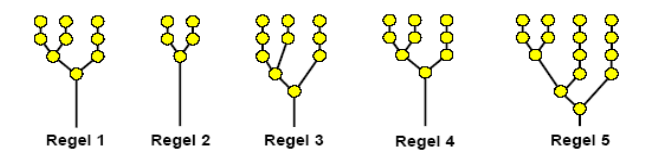
\includegraphics[width=0.8\textwidth]{figures/kap7/rule-mesh.png}
    \caption{Beispiel eines Regelnetzes}
    \label{fig:xps-rule-mesh}
\end{figure}

\begin{figure}[H]
    \centering
    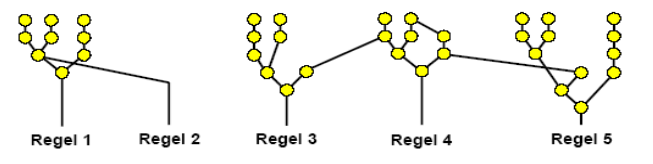
\includegraphics[width=0.8\textwidth]{figures/kap7/combined-rule-mesh.png}
    \caption{Kombinierte Regelnetze}
    \label{fig:xps-rule-mesh-combined}
\end{figure}

\section{Konfliktaufl�sung von Regelsystemen}

In vielen F�llen sind mehrere Regeln anwendbar, so dass sich die Frage stellt, welche Regeln man anwenden sollte. Die Antwort auf diese Frage h�ngt von der Reihenfolge der Regeln in der Regelbasis ab. In kommutativen Systemen kann eine schlechte Wahl der Regeln zu langen L�sungen f�hren. In nicht-kommutativen Systemen kann die Schwierigkeit der Suche aufgrund der R�ckverfolgung exponentiell sein. 

\paragraph{Ansatz 1: Heuristische Regelauswahl}

Wie bei den meisten Suchproblemen k�nnen Heuristiken den Prozess effizienter machen. Ein g�ngiger Ansatz besteht darin, sich an der H�ufigkeit der verwendeten Regel zu orientieren, d. h. jede Regel darf nur einmal verwendet werden. Ansonsten kann es von Vorteil sein, Regeln zu bevorzugen, die auf den neuesten generierten Daten beruhen. Schlie�lich ist es auch m�glich, eine Implementierung zu erstellen, die auf spezifischen Merkmalen des Problems basiert. Das bedeutet, dass Regeln, die mehr mit dem aktuellen Problem zu tun haben, bevorzugt werden.

\paragraph{Ansatz 2: Meta-Regeln}

Metaregeln sind Regeln �ber Regeln. In diesem Fall w�re ein Ansatz, Regeln �ber die Auswahl von Regeln in Form von Regeln zu bilden. Einige Meta-Regeln w�ren zum Beispiel: Regeln mit billigeren Verfahren gegen�ber teuren Verfahren bevorzugen, Regeln mit weniger gef�hrlichen Ans�tzen gegen�ber gef�hrlicheren Ans�tzen bevorzugen, Regeln von Experten gegen�ber Anf�ngern bevorzugen.
\chapter{Formaler Logik}

\section{Wissensrepr�sentation und wissensbasierte Verarbeitung auf der Grundlage formaler Logik}

Es gibt F�lle, in denen Schlussfolgerungen aus Fakten, Gegenst�nden oder Zusammenh�ngen gezogen werden m�ssen. Zum Beispiel manchmal Fragen wie: Hat Objekt A Merkmal B? Oder ist A mit B verwandt? m�ssen beantwortet werden.   Dies kann mit einem System geschehen, das formale Logik verwendet.

Die Idee, die hinter der Funktionsweise eines Logiksystems steht, ist die Definition der anwendungsspezifischen Fakten (durch eine Logiksprache) und die anschlie�ende Einspeisung dieser Definition in einen allgemeinen anwendungsunabh�ngigen Verarbeitungsmechanismus. Der Verarbeitungsmechanismus generiert dann eine L�sung auf der Grundlage der definierten Fakten. Dieser Verarbeitungsmechanismus erfolgt durch logische Schlussfolgerungen und wird auch als Inferenzmechanismus bezeichnet. 

\subsection{Syntax und Semantik einer Logiksprache}

Um Fakten und Zusammenh�nge zu definieren, ist eine formale Sprache notwendig. Die Syntax einer Logiksprache definiert, welche Zeichenketten korrekt ausgedr�ckt werden (auch bekannt als Terme, S�tze, Ausdr�cken oder Formeln).

Bei der Semantik geht es darum, wie die Sprache definiert, unter welchen Umst�nden ein Ausdruck wahr ist.  Semantik legt fest, wie die Sprache definiert, unter welchen Umst�nden ein Ausdruck in der gegebenen "Welt" wahr ist.

Die Aussagenlogik beschreibt Beziehungen zwischen Ausdr�cken, die wahr oder falsch sein k�nnen, und abstrahiert von der nat�rlichen Sprachstruktur der Aussage.

\paragraph{Syntax der Aussagenlogik}

Die in der formalen Sprache ausgedr�ckte Aussagenlogik hat eine lexikalische und eine sturkturelle Komponente. Die lexikalische Komponente besteht aus grundlegenden Symbolen wie Konstanten (TRUE, FALSE), Satzsymbolen (A, B, C), logischen Verkn�pfungssymbolen (\(\wedge \vee \neg \Leftrightarrow \Rightarrow\)) und Klammern. Die Strukturkomponente besteht aus Regeln, die syntaktisch korrekte S�tze (Aussagen) bilden. Ein Beispiel f�r einen Satz ist: \(A \vee \neg B \vee C \wedge D\) was bedeutet: ``A oder nicht B oder C und D''.

\paragraph{Semantik aussagenlogischer Ausdr�cke}

Die Semantik (d.h. die Bedeutung) eines aussagenlogischen Ausdrucks wird als eine Interpretation bezeichnet. Eine Interpretation ist eine Abbildung,\(I\), die S�tze auf ihre Wahrheitswerte abbildet.

\subsection{Begriffe der Aussagenlogik-Syntax}

\paragraph{Literale}

Eine aussagenlogische Variable ist als positives Literal bekannt (z.B:~\(A\)), und negierte sind als negative Literale bekannt (z.B:~\(\neg A\)).

\paragraph{Klausel}

Eine Formel, die aus einer Disjunktion von n Literalen besteht, ist eine Klausel (z.B:~\(A \vee \neg B \vee C \wedge D\)). 

\paragraph{Konjunktive Normalform}

Eine Formel, die aus einer Konjunktion von Klauseln besteht, hat die konjunktive Normalform (z.B:~\((A \vee \neg B \vee C \wedge D) \wedge (A \vee C \wedge E) \wedge \neg F\)).

\subsection{Belegung, Modell und Erf�llbarkeit}

Gegeben sei \(\phi\) ein Satz, \(\sigma\) eine Belegung f�r die Aussagevariablen in \(\phi\) und \(I\) eine Interpretationsfunktion mit \(I(\phi) = TRUE\). Dann ist:

\begin{itemize}
    \item \(\phi\) g�ltig unter der Belegung \(\sigma\)
    \item \(\sigma\) ist ein Modell von \(\phi\).
\end{itemize}

Notation daf�r w�re \(\sigma \models \phi\).

Gegeben sei \(\phi\) ein Satz dann ist \(\phi\) erf�llbar genau dann wenn \(\phi\) mindestens ein Modell hat. Eine Menge von \(F\) Formeln ist erf�llbar genau dann wenn eine Belegung \(\sigma\) existiert, unter der alle Formeln \(\phi_i\) aus \(F\) g�ltig sind.    

\section{L�sen von SAT-Problemen mit SAT-Solver}

SAT-Probleme bedeuten boolesche Erf�llbarkeitsprobleme. Solche Probleme k�nnen mit einem SAT-Solver gel�st werde. Dies kann erfolgen, indem einfach boolesche Formeln \(\phi\) an einen SAT-Solver �bergeben werden, der dann nach \(I(\phi)=TRUE\) aufl�st.

\begin{figure}[H]
    \centering
    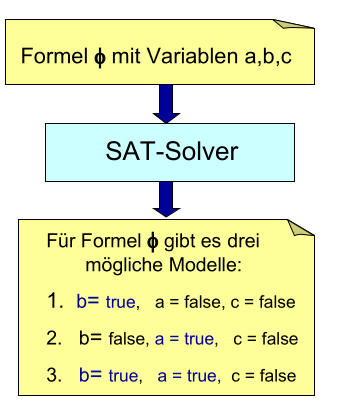
\includegraphics[width=0.4\textwidth]{figures/kap8/SAT-solver.png}
    \caption{Verwendung eines SAT-Solvers}
    \label{fig:using-sat-solver}
\end{figure}

Abbildung~\ref{fig:using-sat-solver} zeigt die Ausgabe der Variablen a,b,c mit der folgenden Formel:

\[ \phi = (a \vee b \vee c) \wedge (a \Rightarrow \neg(a \wedge c)) \wedge (c \Rightarrow (a \wedge c \vee b \wedge c)) \wedge (\neg a \Rightarrow (\neg c \wedge b \vee \neg b \wedge c))\]

Was die folgende Wahrheitstabelle ergibt:

\begin{figure}[H]
    \centering
    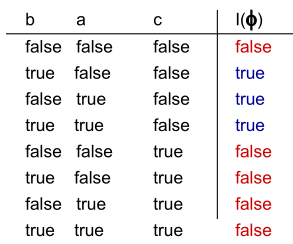
\includegraphics[width=0.4\textwidth]{figures/kap8/truth-table-SAT.png}
    \caption{Wahrheitstabelle des SAT-Problems}
    \label{fig:sat-solver-truthtable}
\end{figure}

Ein Beispiel f�r eine Anwendung eines SAT Solvers ist das Spiel Sudoku. Man kann die Einschr�nkungen der Sudoku-Felder mit einer Logiksprache definieren und dann einen SAT-Solver verwenden, um ein Modell zu finden, das das Problem l�sen kann.

\section{Ausdrucksst�rke Logiksprachen}

Die Aussagenlogik funktioniert in einigen F�llen, ist aber auf die Modellierung von Fakten beschr�nkt. Dies kann zu kompliziert werden, wenn alle strukturellen Beziehungen explizit als Fakten dargestellt werden m�ssen. Mit Aussagenlogik gibt es keine Quantifizierung, keine Relationen und keine Funktionen. Logikprache muss also erweitert werden, um aussagekr�ftiger zu sein.

\subsection{Pr�dikatenlogik 1. Stufe}
\label{section:pl1}
Die logische Sprache wird um Pr�dikate (boole'schen Funktionen), Variablen und Quantoren (erm�glicht es, �ber eine Menge von Objekten mit Hilfe einer Variablen zu sprechen) erweitert.

Pr�dikatenlogik 1. Stufe (First Order Logic) beschreibt Objekte, ihre Eigenschaften und ihre Beziehungen zueinander. Es gibt bei Pr�dikatenlogik auch eine Unterscheidung zwischen Syntax und Semantik.

\paragraph{Syntax: Lexikalischer Teil}

\begin{itemize}
    \item Konstanten-Symbole: TRUE, FALSE, A, B, Hans, Paul\dots
    \item Variablen-Symbole: x, y, \dots
    \item Funktions-Symbole: plus, minus, mul, Vater\_von\dots
    \item Pr�dikaten-Symbole: student, hat\_Computer, P, Q\dots
    \item Logische Verkn�pfungen: \(\vee \wedge \neg \Leftrightarrow \Rightarrow \)
    \item Quantoren: \(\exists , \forall\)
    \item Gleicheit: \(=\)
\end{itemize}

\paragraph{Syntax: Struktureller Teil}

\begin{itemize}
    \item \textbf{Terme:} Konstaten-Symbole, \( f(t_1, t_2, t_3, \dots, t_n) \) wenn \(f\) eine Funktionsymbol und \(t_1\) bis \(t_n\) Terme sind.
    \item \textbf{Atomare Formel:} \(P(t_1, t_2, t_3, \dots, t_n)\) wenn Pr�dikatensymbol \(P\) und \(t_1\) bis \(t_n\) Terme sind.
    \item \textbf{Komplexe Formel:} jede atomare Formel ist eine Formel. Wenn R und S Formeln sind und x ein Variablen-Symbol dann sind folgende Formeln: \(R\), \(\neg R\), \(R \wedge S\), \(R \vee S\). \(R \Rightarrow S\), \(\exists x: R\), \(\forall x:R\)
\end{itemize}

\paragraph{Beispiele von Sachverhalten-Formulierung in Pr�dikatenlogik}

\begin{itemize}
    \item Alle Kinder lieben Eiscreme: \(\forall x:Kind(x) \Rightarrow liebt\_Eiscreme(x)\)
    \item Es gibt einen Baum der Nadeln hat: \(\exists x:Baum(x) \wedge hat\_Nadeln(x)\)
    \item Die Mutter einer Person ist dessen weibliches Elternteil: 
    \[\forall x \forall y : Mutter(x,y) \Leftrightarrow (weiblich(x) \wedge Elternteil(x,y))\]
\end{itemize}

\subsection{Semantik der Pr�dikatenlogik}

Es wird eine Interpretationsfunktion verwendet, die der Aussagelogik �hnelt, aber komplexer ist. Der Wahrheitsgehalt einer Formel wird durch die Struktur, \(S = (U,I)\) bestimmt, wobei U das ``Universum'' (beobachteter Gegenstandsbereich) und I die Interpretationsabbildung (die Bestandteile einer Formel, die die Objekte und Relationen im Gegenstandsbereich abbildet) sind.

\section{Vertiefung: Prolog ausprobieren}

Mit Hilfe der Online-Prolog-Umgebung\cite{prolog-online} wurde folgendes ausprobiert, um ein Gef�hl f�r die Programmierung in Prolog zu bekommen:

\paragraph{Einfaches Beispiel f�r Beziehungen mit Prolog}

\begin{lstlisting}
%facts
likes(dan,sally).
likes(sally,dan).
likes(josh, brittney).
likes(sally, brittney).

hates(josh, dan).
hates(dan, josh).
hates(brittney, sally).

friendship(X,Y):-
    likes(X,Y),
    likes(Y,X).

enemies(X,Y):-
    hates(X,Y),
    hates(Y,X).

misunderstanding(X,Y):-
    hates(X,Y),likes(Y,X);
    hates(Y,X),likes(X,Y);
\end{lstlisting}

\begin{figure}[H]
    \centering
    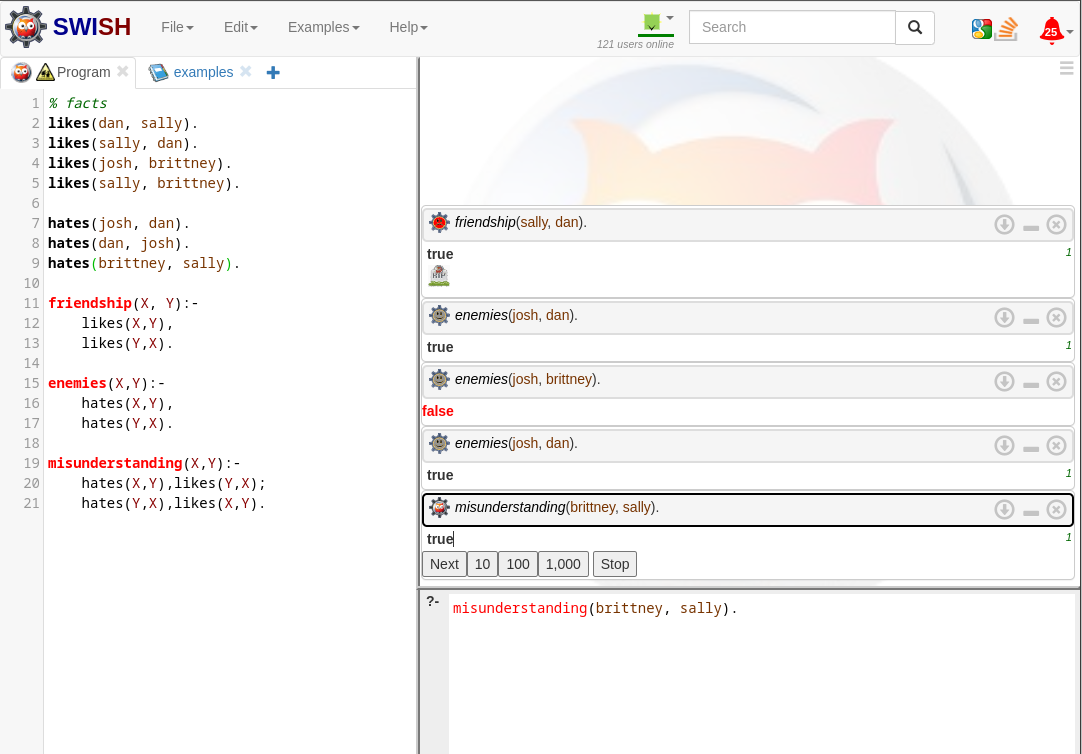
\includegraphics[width=\textwidth]{figures/kap8/prolog-relationships.png}
    \caption{Einfaches Modell von Beziehungen mit Prolog}
    \label{fig:prolog-relationships}
\end{figure}

\paragraph{Ein eher faktenbasiertes Beispiel}

\begin{lstlisting}
fond_of_humans(cat).
fond_of_humans(dog).

comfortable_in_houses(cat).
comfortable_in_houses(dog).

breeds_easily_in_captivity(cat).
breeds_easily_in_captivity(dog).
breeds_easily_in_captivity(chicken).
breeds_easily_in_captivity(cow).
breeds_easily_in_captivity(horse).
breeds_easily_in_captivity(ox).

grows_quickly(chicken).
grows_quickly(cow).

useful_animal(horse).
useful_animal(ox).
useful_animal(dog).

is_pet(X):-
    fond_of_humans(X),
    comfortable_in_houses(Y).

is_farmed(X):-
    breeds_easily_in_captivity(X),
    grows_quickly(X).

is_work_animal(X):-
    breeds_easily_in_captivity(X),
    useful_animal(X).
\end{lstlisting}

\begin{figure}[H]
    \centering
    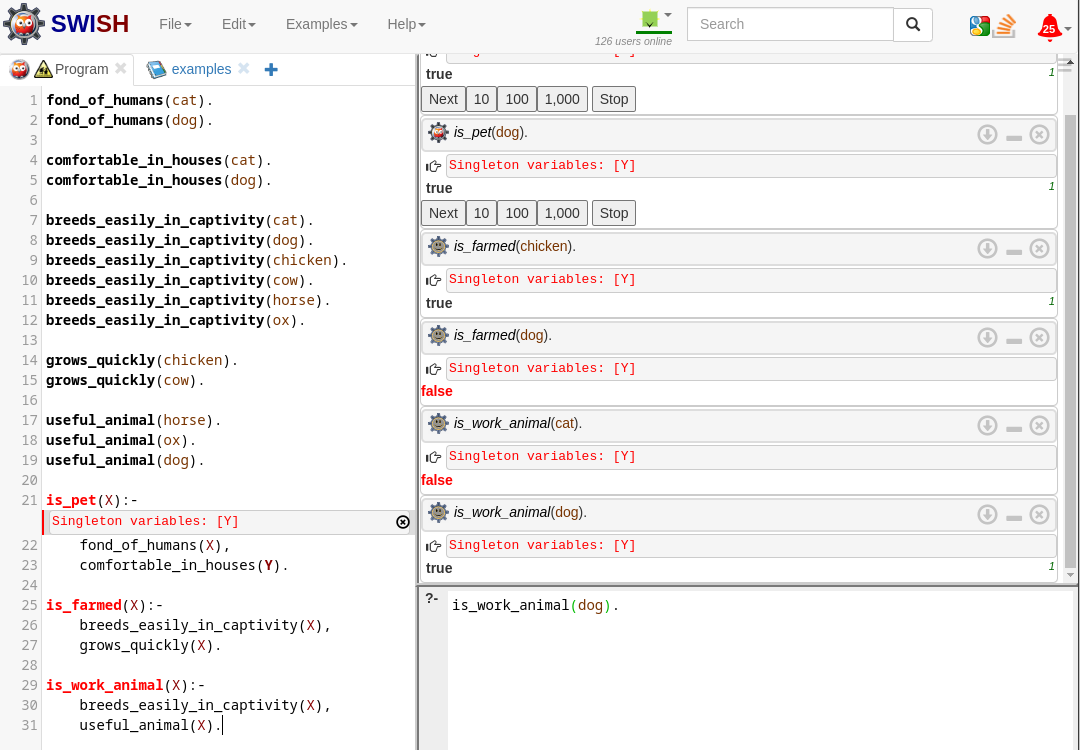
\includegraphics[width=\textwidth]{figures/kap8/prolog-animals.png}
    \caption{Einfaches Modell von Tieren mit Prolog}
    \label{fig:prolog-animals}
\end{figure}
\chapter{Verfahren zur Handlungsplanung}

\section{Einf�hrung in die Planung}

\paragraph{Plan vs Planen}

Wenn es um Handlungsplanung geht, ist es wichtig, den Unterschied zwischen einem Plan und einer Planung zu kennen. Ein \textbf{Plan} ist eine Struktur, die Darstellungen von Aktionen und Zielen enth�lt, die verwendet werden, um �ber die Wirkung zuk�nftiger Aktionen zu urteilen und die zielgerichtete Ausf�hrung von Aktionen zu beeinflussen. Das \textbf{Planen} ist die Generierung von Handlungsabl�ufen, die von einer gegebenen Situation ausgehen und zu einer gew�nschten Zielsituation f�hren.

\paragraph{Arten von Pl�nen}

Planungsaufgaben sind oft komplexer Natur und erfordern die Verarbeitung unterschiedlichster Informationen. Es gibt im Allgemeinen drei Arten von Pl�nen, lineare Pl�ne, nichtlineare Pl�ne und hierarchisch strukturierte Pl�ne. Ein \textbf{linearer Plan} ist eine Abfolge von Handlungen, die befolgt werden k�nnen, um das Ziel zu erreichen. Ein \textbf{nichtlinearer Plan} ist eine Menge von Aktionen, die nur teilweise nach Ausf�hrungszeit geordnet sind, da einige Aktionen parallel ausgef�hrt werden k�nnen. Ein \textbf{hierarchisch strukturierter Plan} ist ein Plan, der aus Teilpl�nen besteht.

\paragraph{Spezifikation einer Planungsaufgabe}

Zur Bearbeitung einer Planungsaufgabe mit einem Computer werden eine geeignete Sprache zur Definition der Aufgabe und ein Planungsalgorithmus zur L�sung der Aufgabe ben�tigt. Die Sprache muss in der Lage sein, die Dom�ne der Aufgabe, diesen Zustand des Suchraums und die erlaubten Aktionen zu definieren. Was den Algorithmus anbelangt, so bestehen die beiden Implementierungsmethoden darin, ein allgemeines Verfahren zu verwenden, z. B. eine Suche mit Backtracking, oder einen f�r die Aufgabe spezifischeren Prozess zu verwenden (der normalerweise effizienter ist).

\section{Planen als logische Inferenz}

\paragraph{Klassisches KI-PLanen: Blocks World}

``Blocks World'' ist ein klassisches Beispiel, wenn es um Planung mit KI geht. In der Welt der Bl�cke gibt es einige identifizierbare Bl�cke, A, B, C, \dots, die nebeneinander liegen oder �bereinander gestapelt sind. Es gibt auch einen Greifer, der einen Block aufnehmen kann, solange kein anderer Block auf dem zu aufnehmenden Block gestapelt ist.

\begin{figure}[H]
    \centering
    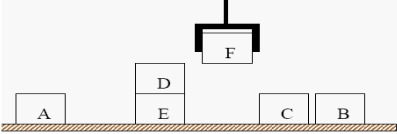
\includegraphics[width=0.7\textwidth]{figures/kap9/blocks-world.png}
    \caption{Darstellung von Blocks World}
    \label{fig:blocks-world}
\end{figure}

Da die Startpositionen und die Zielkonfiguration der Bl�cke im Stil der Pr�dikatenlogik 1. Stufe (siehe Kapitel~\ref{section:pl1}) als Konjunktion von Eigenschaften gegeben sind, wird eine Folge von Aktionen f�r den Greifer gesucht, die die Konfigurations�nderung von der Startposition zur Zielposition bewirken kann.

\paragraph{L�sen mittels logische Inferenz}

Eine M�glichkeit, eine L�sung f�r dieses Problem zu finden, ist das Planen als logische Inferenz. Die klassische Pr�dikatenlogik ist f�r dynamische Prozesse wie diesen nicht geeignet. Um dies zu umgehen, k�nnen Zust�nde, \(s\), als Objekte mit bestimmten Eigenschaften \(P(s)\) und \(Q(s)\) betrachtet werden. Aktion, A kann als eine �bergangsrelation \(A(s_i, s_k)\) gebildet werden, die den Zustand \(s_i\) auf \(s_k\) abbildet. Die Aktionen k�nnen dann als Regeln in der Form:

\[(P(s_i) \wedge A(s_i, s_k)) => Q(s_k)\]

Diese Art der Planung hat viele Vorteile: Die Formulierung des Problems kann sich in diesem Fall auf die Formulierung von Aktionen und den Ziel- und Startzustand beschr�nken und ein allgemeiner Theorembeweiser kann verwendet werden, um das Problem zu l�sen, indem das durch die Inferenzschritte erzeugte Protokoll zur�ckverfolgt wird.

Dieser Ansatz hat jedoch auch einige Nachteile. N�mlich die Tatsache, dass man eine Reihe von Problemen bew�ltigen muss, die mit der Verwendung eines Planoperators einhergehen. Diese Reihe von Problemen besteht im Wesentlichen darin, dass es nicht m�glich ist, die Auswirkungen einer Handlung zu beschreiben, insbesondere in der realen Welt, wenn einige Handlungen fehlschlagen. Au�erdem ist die Planerstellung nicht besonders effizient, da sie einen allgemeinen L�ser verwendet.

\section{STRIPS-Planer}

STRIPS steht f�r ``Stanford Research Institute Problem Solver''. In STRIPS wird eine Planungsaufgabe als \((S, O, F)\) dargestellt, wobei \(S\) und \(F\) eine Menge von Pr�dikaten sind. \(S\) beschreibt den Startzustand, \(F\) den Zielzustand und \(O\) ist eine Menge von STRIPS-Operatorschemata.

Ein STRIPS-Planoperator ist der Tripel \(Op = (P, D, A)\). \(P\) sind die Vorbedingungen (engl. Preconditions) die gelten m�ssen, damit Op auf eine Konstellation anwendbar ist. \(D\) ist die Menge der wegfallenden Fakten (Delete List) nach einer Ausf�hrung von Op. \(A\) ist die Menge der neuen Fakten (Add List), die nach einer Ausf�hrung von Op gelten.

\paragraph{Beispiele f�r eine Operator-Schema mit Variablen}

Ausf�hrung von \(pickup(x)\), einen Block vom Tisch aufheben:

\begin{itemize}
    \item \(P:{OnTable(x), Clear(x), Handempty}\)
    \item \(D:{Holding(x), Clear(y), Handempty}\)
    \item \(A:{Holding(x)}\)
\end{itemize}

Ausf�hrung von \(putdown(x)\), einen Block, den der Greifer gerade h�lt, auf den Tisch legen:

\begin{itemize}
    \item \(P:{Holding(x)}\)
    \item \(D:{Holding(x)}\)
    \item \(A:{OnTable(x), Clear(x), Handempty}\)
\end{itemize}

Ausf�hrung von \(stack(x, y)\), was bedeutet, dass Block X auf Block Y gestapelt wird:

\begin{itemize}
    \item \(P:{Holding(x), Clear(y)}\)
    \item \(D:{Holding(x), Clear(y)}\)
    \item \(A:{Handempty, Clear(x), On(x,y)}\)
\end{itemize}

Ausf�hrung von \(unstack(x, y)\), was bedeutet, dass Block x von der Oberseite von Block y aufgenommen wird:

\begin{itemize}
    \item \(P:{Handempty, Clear(x), On(x,y)}\)
    \item \(D:{Handempty, Clear(x), On(x,y)}\)
    \item \(A:{Holding(x), Clear(y)}\)
\end{itemize}

\paragraph{Ausf�hrung einer Aktion mittels STRIPS}

\begin{enumerate}
    \item Unifiziere der Vorbedingungen der Aktion mit der aktuellen Zustandsbeschreibung.
    \item Instantiiere die Add- und Delete-Listen mit dem gefundenen Unifikator.
    \item L�sche die Atome der instantiierten Delete-Liste aus der aktuellen Zustandsbeschreibung.
    \item F�ge die Atome der Add-Liste der neuen Zustandsbeschreibung hinzu.
\end{enumerate}

\section{}
\chapter{Darstellung und Verarbeitung von unsicherem Wissen}

Im Alltag gibt es viele Beispiele f�r unsicheres Wissen: das Wetter von morgen, die Karten des Gegners beim Kartenspiel oder die Gewinnzahlen im Lotto. Solche Ungewissheit kommt auch in der KI vor, und es gibt viele Techniken, um mit diesem unsicheren Wissen umzugehen und sie zu verarbeiten.

\section{Einf�hrung in unsicheres Wissen}

Die meisten �u�erungen unsicheren Wissens sind auf unvollst�ndiges Wissen oder Zuf�lligkeit zur�ckzuf�hren. Dieses unvollst�ndige Wissen hat paar m�gliceh Quellen: Ein Ausdruck kann sich auf ein zuk�nftiges Ereignis beziehen, aufgrund von Leistungseinschr�nkungen auf Sch�tzungen beruhen oder aus einer unvollst�ndigen Modellierung eines Kontexts in einer Dom�ne gefolgert werden, was alles zu Unsicherheit f�hren kann.

Unsicherheit l�sst sich nicht mit klassischen Logik (wie Aussagenlogik oder PL1, etc) oder mit klassischen Wenn-dann-Regeln formulieren. Dies wirft nat�rlich die Frage auf, wie wir Unsicherheit beschreiben und f�r Schlussfolgerungen und Inferenzen nutzen k�nnen?

\paragraph{Modellierung von unsicherem Wissen}

Die Modellierung unsicheren Wissens kann auf verschiedene Arten erfolgen. Ein Ansatz besteht darin, Ausdr�cken Wahrscheinlichkeiten zuzuweisen und diese Wahrscheinlichkeiten zu verwenden, wenn Schlussfolgerungen gezogen werden. Ein Ansatz besteht darin, Ausdr�cken Wahrscheinlichkeiten zuzuweisen und diese \textbf{Wahrscheinlichkeiten} zu verwenden, wenn Schlussfolgerungen gezogen werden. Ein anderer Ansatz w�re die Zuweisung von \textbf{``Sicherheitswerte''}, um auszudr�cken, wie sicher man sich einer bestimmten Fakt oder Regel ist. Schlie�lich kann Unsicherheit auch unter Verwendung \textbf{nicht monotoner Schlie�en} und \textbf{Default-Logik} modelliert werden, was bedeutet, bestimmte ``Defaults'' anzunehmen, die sp�ter widerrufen werden k�nnen.

\section{Einschub: Wahrscheinlichkeitsrechnung}

Sei A ein Ereignis, das eintreten oder nicht eintreten kann, lautet die Definition der Wahrscheinlichkeit \(P(A) \in [0, \dots, 1]\):

\[ P(A) = \frac{\textnormal{Anzahl der F�lle in denen A eintritt (g�nstige F�lle)}}{\textnormal{Gesamtzahl der m�glichen F�lle, in denen A eintreten kann}} \]

Es gibt zwei Arten von Wahrscheinlichkeiten, \textbf{a priori Wahrscheinlichkeit} und \textbf{bedingte Wahrscheinlichkeit}. A priori Wahrscheinlichkeit, \(P(A)\) dr�ckt aus, wie wahrscheinlich das Ereignis A eintreten wird. Bedingte Wahrscheinlichkeit, \(P(B | A)\), dr�ckt aus, wie wahrscheinlich das Ereignis B in Abh�ngigkeit von der Wahrscheinlichkeit des Ereignisses A eintritt.

\paragraph{Bedingte Wahrscheinlichkeit}

Definition bedingte Wahrscheinlichkeit:

\[P(B|A) = \frac{P(A \cap B)}{P(A)}\]

sowie:

\[P(A|B) = \frac{P(A \cap B)}{P(B)}\]

Bei der Berechnung von Wahrscheinlichkeiten ist zu unterscheiden zwischen dem Fall, dass ein Ereignis von einem anderen abh�ngig ist, und dem Fall, dass die beiden Ereignisse unabh�ngig voneinander sind. 

Die Wahrscheinlichkeit, zwei gleichfarbige Kugeln aus einer Urne mit gemischten Kugeln auszuw�hlen, ist ein klassisches Beispiel f�r einen Fall, in dem das Ereignis A, das die erste Kugel ausw�hlt, sich direkt auf die Wahrscheinlichkeit von B auswirkt, eine zweite Kugel der gleichen Farbe auszuw�hlen. Andererseits ist die Wahrscheinlichkeit, zwei gleiche Augenzahlen zu w�rfeln, unabh�ngig vom ersten Wurf.

\paragraph{Totale Wahrscheinlichkeit}

Zerlegt man den Ereignisraum G in die paarweise disjunkte Mengen (disjunkt = sich gegenseitig ausschlie�ende Ereignisse) \(A_1\) bis \(A_n\), und gilt f�r jedes \(A_i\) dass \(P(A_i) > 0\), so l�sst sich f�r ein belibiges Ereignis B die Wahrscheinlichkeit \(P(B)\) berechnen durch:

\[P(B) = \sum_{i=1}^{n} P(B \cap A_i) = \sum_{i=1}^{n} P(A_i) * P(B | A)\]

\paragraph{Bayes'sche Formel}

Seien \(A_1\) bis \(A_n\) eine disjunkte Zerlegung des Ereignisraums \(G\) und sei \(B\) mit \(P(B) \neq 0 \) ein bereits eingetretenes Ereignis. Dann kann man ein \(P(A_i | B)\) wie folgt berechnen:

\[ P(A_i | B) = \frac{P(A_i) * P(B | A_i)}{\sum P(A_k) * P(B | A_k)} \textnormal{ f�r } 1 \le i \le n \textnormal{ und } 1 \le k \le n\]

\section{Probabilistisches Schlussfolgern}

Unter Verwendung der Regeln der Wahrscheinlichkeitsrechnung ist es m�glich, Anwendungsmodelle zu erstellen, in denen verschiedene probabilistische Schlussfolgerungen unterscheidet werden.

Aus Fakten mit a priori bedingter Wahrscheinlichkeit \(P(B | A_i)\) kann auf die Wahrscheinlichkeit des Ereignisses B geschlossen werden. Aus dem Eintreten des Ereignisses B kann nach der Bayes-Formel die wahrscheinlichste Ursache von B bestimmt werden.

Bayes'sche Graphen werden in der Praxis verwendet, wobei kausale Beziehungen als bedingte Wahrscheinlichkeiten dargestellt werden. Zur Modellierung von Ereignissen werden sogenannte Zufallsvariablen und Wahrscheinlichkeitsverteilungen verwendet.

Zufallsvariablen sind Variablen die durch Zufallsprozesse zugewiesen werden. Es gibt drei Typen: boolesch (z.B M�nzwerf), diskret (z.B W�rfelwurf) und kontinuierlich (z.B Temperatur Morgen).

Eine Wahrscheinlichkeitsverteilung ist eine Zufallsvariable mit m�glichen Werten von 0 bis 1. Dieser Wert wird verwendet, um die Wahrscheinlichkeit darzustellen, dass ein Ereignis eintritt, wobei 1 eine Wahrscheinlichkeit von 100\% und 0 eine Wahrscheinlichkeit von 0\% darstellt.

\section{Bayes'schen Netze}

Ein Bayes'schen Netz ist ein Graph, in dem Zufallsvariablen die Knoten und die bedingten Wahrscheinlichkeiten zwischen den Variablen die Kanten sind.

\paragraph{Aufabau eines Bayes'schen Netzes}

\begin{enumerate}
    \item Um ein Bayes'sches Netz aufzubauen, m�ssen zun�chst alle Zufallsvariablen und ihre Wertebereiche f�r eine bestimmte Anwendung identifiziert werden.
    \item Alle Zufallsvariablen werden in einem Netzwerk so angeordnet, dass alle Klauselabh�ngigkeiten zwischen Variablen durch Kanten dargestellt werden.
    \item F�r Variablen, die nicht voneinander abh�ngig sind, soll eine a priori Wahrscheinlichkeitsverteilung bestimmt werden.
\end{enumerate}

Wenn eine Variable \(Y\) direkt von den Variablen \(X_1\) bis \(X_n\) abh�ngt, m�ssen die bedingten Wahrscheinlichkeiten f�r alle Werte von \(i\) bestimmt werden.

\paragraph{Modellieren mit Bayes'schen Netzen}

Um die Modellierung mit einem Bayes'schen Netz besser zu erkl�ren, wird folgender Fall betrachtet:

\textit{Wenn Hans anruft (H), oder wenn Maria anruft (M), dann gab es einen Alarm (A), der durch einen Einbruch (E), einen Sturm(S), oder durch beides (E und S) ausgel�st wurde, wobei folgende a-priori Wahrscheinlichkeitsverteilungen bekannt seien:}

\begin{itemize}
    \item \(P(E) = 0.02\), \(P(\neg E) = 0.98\) 
    \item \(P(S) = 0.02\), \(P(\neg S) = 0.98\) 
    \item \(P(A)\) in Abh�ngigkeit von S und E:
\end{itemize}

\begin{table}[H]
    \centering
    \begin{tabular}{|l|l|l|l|}
    \hline
    \textbf{x1} & \textbf{x2} & \textbf{x3} & \textbf{Test} \\ \hline
    1           & 1           & 1           & nein          \\ \hline
    1           & 1           & 2           & nein          \\ \hline
    1           & 2           & 2           & nein          \\ \hline
    1           & 2           & 1           & nein          \\ \hline
    2           & 2           & 1           & ja            \\ \hline
    \end{tabular}
\end{table}
\chapter{Einf�hrung in Maschinelles Lernen}

Ein Computerprogramm lernt aus Erfahrung E in Bezug auf eine Menge von Aufgaben T und ein Leistungsma� P, wenn sich seine Leistung bei den Aufgaben in T, gemessen durch P, mit der Erfahrung E verbessert.

\section{Lernf�higen Systeme}

Ein lernf�higes System wertet aufbereitete Daten aus, um relevantes Wissen f�r die Durchf�hrung einer Aufgabe zu extrahieren. Dieses Wissen wird im maschinellen Lernen als ``Modelle'' bezeichnet und entweder deklarativ (symbolisch), numerisch (subsymbolisch) oder prozedural (Programmcode) dargestellt.

Das Lernziel ist, Aufgaben effizienter und mit weniger Fehlern zu l�sen, wenn das Modell verfeinert wird. Es kann auch erw�nscht sein, dass ein maschinelles Lernmodell neue Aufgaben �bernehmen kann, indem es neue Begriffe und ihre Bedeutungen, neue Assoziationen und neue Kausalzusammenh�nge lernt.

\subsection{�berwachtes vs Un�berwachtes Lernen}

Es gibt im Allgemeinen zwei Arten von maschinellem Lernen: �berwachtes Lernen und un�berwachtes Lernen. 

\textbf{Beim �berwachten Lernen} wird zwischen einer Lernphase und einer Testphase unterschieden. In der Testphase existiert ein ``Lehrer'', der den Beispieldatensatz klassifiziert und den Prozess �berwacht. W�hrend des Lernens trainiert sich das Modell anhand des gelabelten Datensatzes des Lehrers, und w�hrend der Testphase verwendet das Modell dann einen noch nicht zuvor gesehenen Datensatz ohne Labels und muss zeigen, wie gut es die Daten klassifizieren kann.

\textbf{Beim un�berwachten Lernen} lernt das Modell selbstst�ndig. Dies kann durch Data Mining erfolgen, indem ein Modell mit Daten ``gef�ttert'' und nach Mustern gesucht wird, oder indem positive oder negative ``Erfahrungen'' verwendet werden, um ein Modell zum Lernen zu bringen. Die Verwendung dieses Ansatzes mit Erfahrungen wird als best�rkendes Lernen bezeichnet, bei dem das Modell basierend auf den Ergebnissen seines Trainings positives oder negatives Feedback erh�lt. Das Modell �ndert sich dann basierend auf dem Feedback.

\subsection{Algorithmische Ans�tze zum maschinellen Lernen}

Es gibt einige Ans�tze f�r maschinelles Lernen, die h�ufig verwendet werden:

\begin{itemize}
    \item \textbf{Induktive Lernans�tze:} Anhand konkreter Beispiele wird der allgemeine Fall abgeschlossen. Ein gutes Beispiel ist das Lernen von Begriffen.
    \item \textbf{Statistiche Ans�tze:} Anhand konkreter Beispiele wird auf die H�ufigkeit des wahrscheinlichsten Falles geschlossen. Beispiele: Klassifikation mit ``ZeroR'', ``Naive-Bayes''.
    \item \textbf{Geometrische Ans�tze:} Betrachte Datens�tze als Punkte in einem mehrdimensionalen Koordinatenraum und finde Muster in den Positionen der Datenpunkte. Beispiele: Regression, Support-Vector-Machines.
    \item \textbf{Informationstheoretische Ans�tze:} Einen Datensatz so in Teilmengen aufteilen, dass sich die Teilmengen m�glichst stark voneinander unterscheiden. Beispiele: EM-Clustering, Entscheidungsbaum-Lerner.
    \item \textbf{Symbolisch vs  Subsymbolisch Ans�tze:} 
    \begin{itemize}
        \item Symbolisch: Das erlernte Wissen wird symbolisch dargestellt, z. B.: eine Menge von Regeln, pr�dikatenlogische Formeln, Entscheidungsb�ume etc.
        \item Subsymbolisch/Nueronal: Wissen wird nicht symbolisch gespeichert. z.B: Nueronale Netze, man lernt numerische Gewichte-
    \end{itemize}
    \item \textbf{Pipeline Ansatz (klasssich):} Der Lernprozess wird in verschiedene Schritte unterteilt und mit speziellen Techniken bearbeitet.
    \item \textbf{End-to-End learning/ black-box KI:} Der Lernprozess ist nicht in viele Schritte unterteilt. Stattdessen wird ein tiefes neurales Netz verwendet.
    \item \textbf{Transfer Learning:} Unter Verwendung von Daten aus Quelle A soll eine Schlussfolgerung von Dom�ne B gefunden. Dies geschieht, wenn zu wenige Datens�tze zum Trainieren f�r Dom�ne B vorhanden sind. Dies wird angewendet, indem ein geeigneter Indikator im Datensatz f�r A ausgew�hlt wird, der f�r Dom�ne B verwendet werden kann.
    \item \textbf{Lernen durch Vergleichen, Ausz�hlen und aufteilen von Datens�tzen:} Der Algorithmus durchl�uft den Datensatz und versucht mit einem deterministischen Programm, das Lernziel zu erreichen. Beispiele: Naive Bayes, Entscheidungsbaum-Lerner.
    \item \textbf{Iterative Lernverfahren/ Lernen in Epochen:} Der Lernprozess durchl�uft den Datensatz mehrmals, um das Modell iterativ zu verfeinern. Beispiele: Neuronale Netze, Q-Learning, Regressionsverfahren mit mehreren Variablen.
\end{itemize}

\section{Lernen auf der Grundlage von Daten}

Beim maschinellen Lernen sind \textbf{Daten} grunds�tzlich alle maschinenlesbaren digitalen Darstellungen von Informationen. Ein \textbf{Datensatz} ist eine Struktur in Form von \(d=[d1, ..., dn]\), die aus mehreren Daten erstellt wird. Eine Sammlung von Datens�tzen, die von maschinellen Lernprogrammen verarbeitet werden sollen, werden als \textbf{Datenkorpus} bezeichnet.

\subsection{Einf�hrung in Datens�tzen}

\paragraph{Format eines Datensatzes}

Das Format eines Datensatzes h�ngt von der Art der zu verarbeitenden Daten ab. F�r Datens�tze mit booleschen Typen, nominalen oder numerischen Typen oder Zeitstempeln sind die gebr�uchlichsten Datenformate Comma Seperated Values (CSV), Attribute-Relation-File-Format (ARFF), LIPSVM und JSON.

\paragraph{Arten von Merkmalen}

Bei der Arbeit mit Datens�tzen sind vor allem die im Datensatz gespeicherten Merkmale zu beachten. Es gibt verschiedene Arten von Merkmalen, und die Art beeinflusst die Art der Verarbeitung, die durchgef�hrt werden kann:

\begin{itemize}
    \item \textbf{Nominale Merkmale:} Merkmale, die f�r die Anwendung nicht in eine bedeutungstragende Orndnung gebracht werden konnten. Beispiele: Bool=\{True, False\}, Farbe=\{Rot, Gr�n, Blau\}, Geschlecht=\{w, m, d\}
    \item \textbf{Ordinale (geordnete) Merkmale:} Merkmale, die f�r die Anwendung in eine bedeutungstragende Orndnung gebracht werden k�nnen. Beispiele: Wochentage=\{Mon, Di,  Mi, \ldots\}, Noten=\{sehr gut, gut, \ldots\}
    \item \textbf{Numerische Merkmale:} Die Merkmale sind Zahlenwerte, die einen metrischen Abstand definieren k�nnen. Beispiele: Gr��e, Gewicht, Preis
\end{itemize}

\subsection{Bearbeiten mit Merkmalen}

\paragraph{Vergleich von bin�ren Merkmalen}

Gegeben seien zwei Objekte X, Y mit bin�ren Eigenschaften \(b_1, \ldots\, b_k\). Folgende Variablen werden verwendet:

\begin{itemize}
    \item \textbf{pp=} Anzahl positiver Merkmalen, die sich auf beide Objekte beziehen.
    \item \textbf{pn=} Anzahl von Merkmalen, die sich positiv auf X, aber negativ auf Y beziehen.
    \item \textbf{np=} Anzahl von Merkmalen, die sich negativ auf X, aber positiv auf Y beziehen.
    \item \textbf{nn=} Anzahl negative Merkmalen, die sich auf beide Objekte beziehen.
\end{itemize}

Um den Abstand zwischen zwei Objekten zu berechnen, die diese bin�ren Eigenschaften teilen, kann das Folgende verwendet werden:

\emph{Hamming Distanz:}

\[D_{Ham} (x,y) = pn + np\]

\emph{Simple Matching Distanz:}

\[D_{SMD} (x,y) = \frac{pn + np}{pp+pn+np+nn}\]

\emph{Jaccard Distanz:}

\[D_{JD} (x,y) = \frac{pn + np}{pp+pn+np}\]

\paragraph{Vergleich von nominalen Merkmalen}

Das Problem mit nominalen Merkmalen ist, dass es nicht m�glich ist, sie sinnvoll in eine Rangfolge zu ordnen. Um dies zu l�sen, kann die nominalen Merkmalen binarisiert werden, indem man f�r jeden m�glichen Merkmalswert ein bin�res Merkmal zuordnet.

Zum Beispiel f�r den Familienstand von zwei Personen, \(P_1, P_2\), k�nnen drei boolesche Attribute zugeordnet werden:-

\[ledig(P) -> \{TRUE, FALSE\}\]

\[verheiratet(P) -> \{TRUE, FALSE\}\]

\[geschieden(P) -> \{TRUE, FALSE\}\]

Und jetzt k�nnen die gleichen Methoden f�r bin�re Merkmale wiederverwendet werden.

\paragraph{Vergleich von ordinalen Merkmalen}

F�r ordinale Merkmale \(m \in \{o_1, o_2, \ldots, o_m\}\) ist der Ansatz einfacher. Es m�ssen lediglich die Rangordnungen der Elemente ermittelt werden und als Differenz der Rangordnungen kann die Distanz berechnet werden:

\[D_m(X_m, Y_m) = | Rang(X_m) - Rang(Y_m) |\]

\paragraph{Vergleich von metrischen Merkmalen}

F�r diesen ist der Ansatz �hnlich wie bei nominalen Merkmalen, da die Differenz zwischen ihnen berechnet wird:

\[D_m(X_m, Y_m) = | X_m - Y_m |\]

\subsection{Auswahl von Merkmalen}

Es ist wichtig, die richtigen Merkmale f�r die Aufgabe auszuw�hlen. Generell sollte man Merkmale w�hlen, die f�r alle beobachteten Objekte gelten, einfach und zuverl�ssig bestimmt werden k�nnen und f�r die jeweilige Aufgabe relevant sind.

F�r maschinelle Lernanwendungen ist es jedoch gut, so wenige Merkmale wie n�tig zu verwenden, um die Komplexit�t des Modells zu reduzieren. Anhand eines Korrelationsquotienten ist es m�glich, relevante Merkmalspaare in Datens�tzen zu finden.

Vor der Nutzung eines Datensatzes hilft es, eine sogenannte Datenbereinigung durchzuf�hren. Dazu sollte man Ausrei�er oder unplausible Werte eliminieren, die Daten neu strukturieren, um sie an maschinelle Lernalgorithmen anzupassen und fehlende Werte zu behandeln.

\section{}

\section{Lernen anhand von Beispielen}

F�r diese Art des LernensF�r diese Art des Lernens wird eine Menge von Beispielaufgaben in Form von \((a_1,b_1) \ldots (a_n, b_n)\) gegeben. Es wird angenommen, dass die Zuordnung:

\[f(A) \rightarrow B\] 

wobei \(a_i \in A\) und \(b_i \in B\) gilt. Gesucht wird die Funktion \(f(A) \rightarrow B\). Die Funktion \(f\) ist aber unbekannt und ist das Ziel des Trainierens des Modells. Dazu wird eine Funktion 

\[h(A) \rightarrow B\] 

gesucht, die die Funktion \(f\) am besten ann�hert. 

Dies ist eine Form des �berwachten Lernens, da die Beispiele gegeben werden. Die Menge der Beispiele sollte zuf�llig, aber repr�sentativ f�r \(f\) sein.
\chapter{Methoden des maschinellen Lernens}

\section{Klassifikation}

Unter Klassifizierung versteht man das Sortieren von Datens�tzen in geeignete Klassen. Eine Funktion oder ein Programm, das dies ausf�hren kann, wird als Klassifikator bezeichnet. Die Idee beim maschinellen Lernen besteht darin, das Lernen anhand von Beispielen zu verwenden, um einen Klassifikator zu trainieren, der w�hrend seines Trainings noch nicht gesehene Objekte klassifizieren kann.

Diese Art des Lernens ist eine Form von �berwachtem Lernen, bei dem in der Lernphase positive und negative Beispiele gegeben werden. Die Erfahrungen aus der Lernphase werden dann in der Testphase genutzt, in der das Modell versucht, Beispiele zu klassifizieren, die es noch nicht im Trainingsdatensatz gesehen hat.

F�r die Klassifizierung wird ein Merkmal eines Datensatzes ausgew�hlt, das nach dessen m�glichen Auspr�gungen zur Klassifizierung verwendet wird. Dies ist als Zielmerkmal oder Zielattribut bekannt.

\paragraph{Klassifizierungsworkflow}

\begin{enumerate}
    \item Festlegung der Lernaufgabe und der Datenquelle
    \item Preprocessing: Der Datensatz wird in einen Trainingsdatensatz und einen Testdatensatz aufgeteilt. Der Trainingsdatensatz wird dann mit passendem Klassen-Label versehen.
    \item Das Klassifizierte wird dann mit dem Trainingsdatensatz trainiert.
    \item Das Modell wird mit dem Testdatensatz evaluiert.
    \item Nach Tuning finalen Klassifikator anwenden.
\end{enumerate}

\section{Instanzen-basiertes Klassifizieren}

Gegeben seien eine Menge von Beispieldatens�tzen \(d_1 \ldots d_n\), eine Menge von Klassen \(C_1 \ldots C_m\), in die die Datens�tze \(d_1 \ldots d_n\) unterteilt sind, und ein Datensatz \(d_{new}\). Es wird eine passende Klasse \(C_i\) f�r den neuen Datensatz \(d_{new}\) gesucht.

F�r diesen Fall kann ein Ansatz verwendet werden, der als ``k-n�chste-Nachbarn-Verfahren'' bekannt ist. Unter Verwendung dieses Prozesses wird die Anzahl k der n�chsten Nachbarn des neuen Datensatzes verwendet, um zu entscheiden, zu welcher Klasse der neue Datensatz geh�rt.

\paragraph{Ablauf des k-n�chste-Nachbarn-Verfahrens}

\begin{enumerate}
    \item Die Distanzen zwischen dem neuen Datensatz und den Beispieldatens�tzen werden berechnet.
    \item Die k n�chsten Datenpunkte und ihre Klassen werden bestimmt.
    \item Der neue Datensatz wird basierend auf der Mehrheitsklasse der k n�chsten Nachbarn entschieden.
\end{enumerate}

\section{Klassifikation mit Entscheidungsb�umen}

\subsection{Erlernen einer Entscheidungs-Regel}
\label{section:oneR}
Gegeben sind \(m\) n-dimensionalte Datens�tze \(d_i = [a_1, a_2, \ldots, a_n]\) einer relationalen Datenbank, die interpretiert werden als Argument-Wertepaare einer n-1 stelligen, 1-wertigen Funktion \(f(a_1, a_2, \ldots, a_{n-1})\). Es wird ein einfacher Klassifikator der Form \textbf{IF} \(a_r = w\) \textbf{THEN} \(a_n = k\) gesucht.

Ein Ansatz daf�r w�re, aus dem Trainingsdatensatz ein Attribut \(a_r\) zu bestimmen, das die beste Vorhersage f�r das Zielattribut \(a_n\) liefert, wenn das Attribut \(a_r\) den Wert \(k\) hat.

\subsection{Erlernen einer Entscheidungs-Baums}

Gegeben sind \(m\) n-dimensionalte Datens�tze \(d_i = [a_1, a_2, \ldots, a_n]\) einer relationalen Datenbank, die interpretiert werden als Argument-Wertepaare einer n-1 stelligen, 1-wertigen Funktion \(f(a_1, a_2, \ldots, a_{n-1})\). Es wird ein aber diesmal eine baumartige Entscheidungsstruktur, der einem Datensatz \(d=[a_1, a_2, \ldots, a_{n-1}]\) der passende Wert des Zielattributs \(a_n\) zuordnet.

Der aus den Beispieldaten erstellte Entscheidungsbaum sollte die Attribute so anordnen, dass: 

\begin{itemize}
    \item alle Beispieldatens�tze korrekt klassifiziert werden k�nnen
    \item die Anzahl der Entscheidungen auf ein Minimum beschr�nkt werden
    \item neue Datens�tze klassifiziert werden k�nnen indem diesen Entscheidungsbaum verwendet wird.
\end{itemize}

Zwei m�gliche Strategien zum Aufbau eines Entscheidungsbaums sind:

\begin{itemize}
    \item \textbf{Strategie 1:} Von der Wurzel ausgehend w�hle stets dasjenige Attribut \(a_i\) als n�chstes Auswahlkriterium, welches von den verbleibenden Beispieldatens�tzen die wenigsten ``fehlklassifiziert''. Das bedeutet, dass der zuvor in Kapitel \ref{section:oneR} beschriebene Ansatz rekursiv angewendet wird, um die Attribute f�r den Entscheidungsbaum auszuw�hlen.
    \item \textbf{Strategie 2:} Aus der Wurzel des Baums wird das Attribut ausgew�hlt, das den gr��ten Informationsgewinn hat. Bei dieser Methode wird eine Gleichung zur Berechnung des Informationsgewinns jedes Attributs (Informationstheorie Shanon 1948) rekursiv verwendet, um die Attribute und die Werte des Entscheidungsbaums auszuw�hlen.
\end{itemize}

\section{Evaluation von Klassifikationen}

Beim maschinellen Lernen ist die Bewertung ein wichtiger Schritt f�r die Auswahl eines Klassifizierungsalgorithmus. Diese Auswertung erfolgt anhand von Testdaten, die nicht f�r das Training verwendet wurden. Ein guter Indikator f�r die G�te eines Klassifikators ist die Anzahl der Testdatens�tze, die der Klassifikator richtig und falsch klassifiziert hat. Dies l�sst sich am besten durch eine Konfusionsmatrix veranschaulichen.

\subsection{Evaluation mittels Konfusionsmatrix}

Bei einer Klassifikationsaufgabe, bei der Datens�tze von \(n\) Klassen \(K_1, \ldots, K_n\) klassifiziert werden, wird folgendes durchgef�hrt:
\begin{enumerate}
    \item Unter Verwendung der Klassen \(K_1, \ldots, K_n\) wird eine Matrix \(M\) konstruiert.
    \item In den diagonalen Feldern (\(K_i, K_i\)) von M wird die Anzahl der korrekt klassifizierten Datens�tze eingetragen.
    \item In den Feldern (\(K_r, K_s\)) wobei \(r \neq s\) wird die Anzahl der falsch klassifizierten Datens�tze eingetragen.
\end{enumerate}

\subsection{Konfusionsmatrix f�r zwei Klassen}

Die Datens�tze bestehen aus zwei Klassen \(K_p = \) Positive und \(K_n = \) Negative. Aus dem Datensatz wird die folgende Konfusionsmatrix konstruiert:

\begin{figure}[H]
    \centering
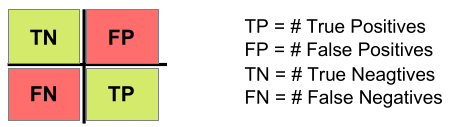
\includegraphics[width=0.6\textwidth]{figures/kap12/2-class-confusion-matrix.png}
    \caption{Konfusionsmatrix f�r zwei Klassen}
    \label{fig:confusion-matrix-2-class}
\end{figure}


Aus dieser Konfusionsmatrix kann das Folgende f�r Klasse \(K_p\) berechnet werden:

\begin{itemize}
    \item Precision, P: \[P = \frac{TP}{TP + FP}\]
    \item Recall, R: \[R = \frac{TP}{TP + FN}\]
    \item Specifity, S: \[S = \frac{TN}{FP + TN}\]
    \item \(F_1\textnormal{-Ma�}\), \(F_1\): \[F_1 = \frac{2*TP}{2*TP+FP+FN}\]
    \item Matthews Correlation Coefficient \[MCC = \frac{TP \times TN - FP \times FN }{\sqrt{(TP+FP)(TP+FN)(TN+FP)(TN+FN)}}\]
\end{itemize}

\subsection{Bewerstungsma�e f�r Klassifikatoren, die numerische Scores liefern}

Einige Klassifikationsaufgaben liefern numerische Werte mit einem Wert von 0 bis 1. Die Idee zur Bewertung dieser Art von Klassifikator besteht darin, die Abweichung der vom Klassifikator erhaltenen Bewertungen im Vergleich zu den tats�chlichen Bewertungen f�r den Datensatz zu berechnen. Es gibt zahlreiche Kennwerte, die auf diesem Prinzip beruhen:

\begin{itemize}
    \item Mittlerer Quadratischer Fehler (MSE): \[MSE = \frac{(p_1 - a_1)^2 + \ldots + (p_n - a_n)^2}{n}\]
    \item Wurzel aus MSE (RMSE): \[RMSE = \sqrt{\frac{(p_1 - a_1)^2 + \ldots + (p_n - a_n)^2}{n}}\]
\end{itemize}

\section{Fehlerquellen f�r maschinelles Lernen}

\begin{itemize}
    \item \textbf{Overfitting:} �beranpassung tritt auf, wenn ein Modell zu gut f�r die Trainingsdaten trainiert wurde. W�hrend des Trainings, um die besten Ergebnisse des Klassifikators beim Testen zu erhalten, wurde m�glicherweise die Varianz eines wichtigen Merkmals �bersch�tzt. Wenn dies geschieht, kann der Klassifikator beim Testen als sehr genau bewertet werden, wird aber neue Daten falsch klassifizieren.
    \item \textbf{Modelle mit Bias:} Ein Modell wird biased, wenn der zum Trainieren des Modells verwendete Datensatz nicht repr�sentativ f�r die tats�chliche Aufgabe war. Das kann viele Ursachen haben, vielleicht wurden Daten aus der falshen Zielgruppe verwendet, oder es wurden nur Profile mit einem bestimmten Feature genommen oder vielleicht war ein Sensor bei der Erfassung der Daten defekt.
    \item \textbf{Overfitting plus Bias:} Wenn ein Klassifikator mit mehreren Datens�tzen trainiert wird und die Leistung der Klassifikatoren gemessen wird, sollte es keine gro�e Varianz geben. Wenn die Varianz hoch ist, bedeutet dies, dass der Klassifikator stark auf kleine �nderungen in den Daten reagiert.
\end{itemize}

\section{Vertiefung: Klassifikatoren Trainieren mit Python}
\label{section:classifier-project}
Um den gesamten Prozess des maschinellen Lernens besser zu verstehen, wurde ein kleines Projekt zum Trainieren eines Klassifikators durchgef�hrt. Dieses Beispiel basiert auf einem Online-Artikel von Medium\cite{classification-online}. In diesem Beispielprojekt werden die �blichen Schritte zur Durchf�hrung von maschinellem Lernen befolgt:
\begin{enumerate}
    \item Data-Preprocessing.
    \item Aufteilen des Datensatzes in Trainings- und Testdatens�tze.
    \item Trainieren des Modells Trainieren der Modelle (eines mit einem Kneighbors-Algorithmus und eines mit einem Entscheidungsbaum).
    \item Klassifikatoren auswerten
\end{enumerate}

In dieser Trainingsaufgabe wird das Modell mit einem Bankdatensatz von Kaggle\cite{kaggle-dataset} darauf trainiert, abh�ngig von einigen Attributen vorherzusagen, ob jemand eine Einzahlung t�tigen wird oder nicht.

\subsection{Data Pre-Processing}

Im Vorverarbeitungsschritt entf�llt die Spalte ``duration'', da diese laut Dokumentation erst verf�gbar ist, nachdem die Label-Spalte bekannt ist. Danach werden die Daten skaliert, um zu vermeiden, dass Ausrei�erdaten das Modell erheblich beeintr�chtigen, und schlie�lich werden die Daten zur einfacheren Verarbeitung mit einer One-Hot-Codierung codiert.

\begin{lstlisting}[language=python]
# load dataset
df_bank = pandas.read_csv('dataset/bank.csv')

# drop duration column
df_bank = df_bank.drop('duration', axis=1)

# create a copy
df_bank_ready = df_bank.copy()

# scaling numberic data to avoid significant outlier presence
scaler = StandardScaler()
num_cols = ['age', 'balance', 'day', 'campaign', 'pdays', 'previous']
df_bank_ready[num_cols] = scaler.fit_transform(df_bank[num_cols])

# Encoding categorical data
encoder = OneHotEncoder(sparse=False)
cat_cols = ['job', 'marital', 'education', 'default', 'housing', 'loan', 'contact', 'month', 'poutcome']

# Encode Categorical Data
df_encoded = pandas.DataFrame(encoder.fit_transform(df_bank_ready[cat_cols]))
df_encoded.columns = encoder.get_feature_names(cat_cols)

# Replace Categotical Data with Encoded Data
df_bank_ready = df_bank_ready.drop(cat_cols ,axis=1)
df_bank_ready = pandas.concat([df_encoded, df_bank_ready], axis=1)

# Encode target value
df_bank_ready['deposit'] = df_bank_ready['deposit'].apply(lambda x: 1 if x == 'yes' else 0)
\end{lstlisting}

\subsection{Splitting the datasets}

Die Daten werden in Trainings- und Testdatens�tze aufgeteilt, wobei 80\% der Daten f�r das Training und 20\% f�r Tests verwendet werden.

\begin{lstlisting}[language=python]
# Select Features
feature = df_bank_ready.drop('deposit', axis=1)

# Select Target
target = df_bank_ready['deposit']

# Set Training and Testing Data
from sklearn.model_selection import train_test_split
X_train, X_test, y_train, y_test = train_test_split(feature , target, 
                                                    shuffle = True, 
                                                    test_size=0.2, 
                                                    random_state=1)

\end{lstlisting}

\subsection{Modelling and evaluation}

Anschlie�end erfolgte die Modellierung der beiden Klassifikatortypen und die Auswertung erfolgte anhand einer Reihe von Metriken sowie einer Konfusionsmatrix.

\begin{lstlisting}[language=python]
# Evaluation function
def evaluate_model(model, x_test, y_test):
    from sklearn import metrics

    # Predict Test Data 
    y_pred = model.predict(x_test)

    # Calculate accuracy, precision, recall, f1-score, and kappa score
    acc = metrics.accuracy_score(y_test, y_pred)
    prec = metrics.precision_score(y_test, y_pred)
    rec = metrics.recall_score(y_test, y_pred)
    f1 = metrics.f1_score(y_test, y_pred)
    kappa = metrics.cohen_kappa_score(y_test, y_pred)

    # Calculate area under curve (AUC)
    y_pred_proba = model.predict_proba(x_test)[::,1]
    fpr, tpr, _ = metrics.roc_curve(y_test, y_pred_proba)
    auc = metrics.roc_auc_score(y_test, y_pred_proba)

    # Display confussion matrix
    cm = metrics.confusion_matrix(y_test, y_pred)

    return {'acc': acc, 'prec': prec, 'rec': rec, 'f1': f1, 'kappa':kappa, 'fpr': fpr, 'tpr': tpr, 'auc': auc, 'cm': cm}

# Model training: decision tree
decision_tree_model = tree.DecisionTreeClassifier(random_state=0)
decision_tree_model.fit(x_train, y_train)

# Model training Kneighbors
kneighbors_model = KNeighborsClassifier()
kneighbors_model.fit(x_train, y_train)
\end{lstlisting}

\subsection{Ausf�hren des Projekts}

Das Projekt (vertiefungen-projekte/python/ml-classifier) kann ausgef�hrt werden, indem zuerst die erforderlichen Bibliotheken installiert werden:

\begin{lstlisting}[language=bash]
pip install -r requirements.txt 
\end{lstlisting}

Und danach l�uft es einfach mit Python:

\begin{lstlisting}[language=bash]
classifier-training.py
\end{lstlisting}

Das Ausf�hren erzeugte die folgende Ausgabe:

\begin{lstlisting}
=====================================================
Decision tree classifier
=====================================================
Accuracy: 0.6336766681594268
Precision: 0.6215953307392996
Recall: 0.598314606741573
F1 Score: 0.6097328244274809
Cohens Kappa Score: 0.2648219403033133
Area Under Curve: 0.6322045136712157
Confusion Matrix:
    [[776 389]
    [429 639]]
=====================================================
K nearest neighbors classifier
=====================================================
Accuracy: 0.6869682042095835
Precision: 0.6981740064446831
Recall: 0.6086142322097379
F1 Score: 0.6503251625812906
Cohens Kappa Score: 0.3693851405429406
Area Under Curve: 0.7323909758724342
Confusion Matrix:
    [[884 281]
    [418 650]]
\end{lstlisting}
\chapter{Data Mining und �berwachtes Lernen}

\section{Ziele beim Data Mining}

Data Mining ist der Prozess des Extrahierens und Entdeckens von Mustern in einer Datensammlung (Datenbank mit Datens�tzen). Es gibt einige Ans�tze, die f�r das Data Mining angewendet werden k�nnen. 

Bei der \textbf{Clusteranalyse} wird eine Menge von Objekten so aufgeteilt, dass Objekte in derselben Gruppe (Cluster genannt) einander �hnlicher sind als denen in anderen Gruppen (Clustern).

Abgesehen davon ist es auch m�glich, in einem Datensatz nach \textbf{Assoziationsregeln zu finden}. Beispielsweise kann es wertvoll sein zu wissen, welche Merkmalskombinationen h�ufiger vorkommen.

Dar�ber hinaus k�nnen Assoziationsregeln durch \textbf{Frequent Pattern Mining} verallgemeinert werden.

Abschlie�end werden mittels \textbf{Faktorenanalyse} korrelierte Merkmale von Datens�tzen analysiert und versucht, diese Merkmale zu ``Faktoren'' zu gruppieren.

\section{Clusteranalyse}

\subsection{Klassifizieren vs Clusteranalyse}

``Clusteranalyse'' und ``Klassifizierung'' m�gen auf den ersten Blick �hnlich erscheinen, aber es gibt einen wesentlichen Unterschied: Bei der Klassifizierung sind die Klassen vordefiniert und den Datens�tzen Klassen zugeordnet, w�hrend beim Clustering der Datensatz nach �hnlichen Merkmalen gruppiert wird, und es ist nicht erforderlich, dass Klassen vordefiniert wurden.

Um ein Clustering zu erreichen, werden �hnliche Objekte zusammen gruppiert, w�hrend un�hnliche Objekte voneinander getrennt werden. Gesucht sind also \(k\) Klassen \(K_1 \ldots K_k\), die alle Objekte richtig gruppieren.

\subsection{Zielsetzung beim Clustering}

\begin{itemize}
    \item In einem Datensatz wird nach der Mindestanzahl von Clustern gesucht.
    \item Objekte im selben Cluster m�ssen so �hnlich wie m�glich sein.
    \item Objekte im selben Cluster m�ssen so �hnlich wie m�glich sein.
    \item Eventuell sollten die Cluster auch hierarchisch geordnet werden k�nnen.
\end{itemize}

\subsection{Clusterbildungverfahren}

Bei der Auswahl von Merkmalen sollen die Merkmalen, die f�r alle Objekte auch Merkmalsauspr�gungen aufweisen werden, die mit vertretbarem Aufwand ermittelt werden k�nnen.

\paragraph{Typen von Merkmalen:}
\begin{itemize}
    \item Nominale Merkmale: z.B Namen, Farbe, \ldots
    \item Ordinale (geordnete) Merkmale: z.B Wochentage, Schulnoten, \ldots
    \item Metrische Merkmale: z.B Gr��e, Gewicht, Preis, \ldots
\end{itemize}

Die Clusteranalyse kann entweder hierarchisch oder durch Partitionierung angegangen werden. Beim hierarchischen Ansatz gibt es zwei M�glichkeiten: Top-Down, das mit einer Klasse beginnt, die sp�ter in mehrere Klassen aufgeteilt wird, oder Bottom-Up, das darin besteht, Klassen zusammenzufassen. Der Partitionierungsansatz gruppiert Objekte durch Umgruppierung. Jede Klasse hat einen vordefinierten "Kristallisationskern". Jedes neue Objekt wird anhand seiner Entfernung zum n�chsten Kristallisationskern eingeordnet.

\paragraph{Hierarchisches Clustering}

Beim hierarchischen Clustering geht es einfach darum, den Abstand zwischen Datenpunkten zu bestimmen und Objektpaare mit minimalen Abst�nden zwischen ihnen zu finden. Dies wird kontinuierlich durchgef�hrt, bis eine Hierarchie aufgebaut ist.

\begin{figure}[H]
    \centering
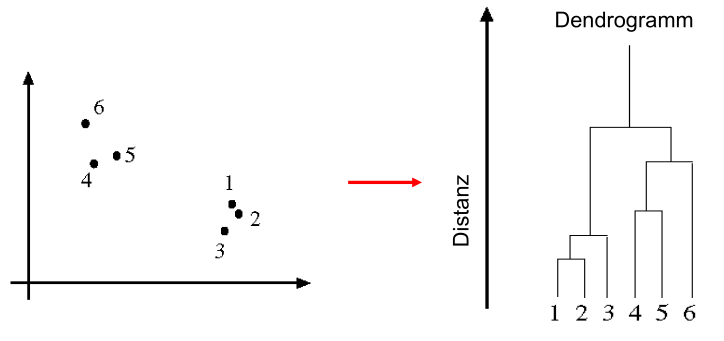
\includegraphics[width=0.9\textwidth]{figures/kap13/hierarchy-clustering.png}
    \caption{Hierarchisches Clustering}
    \label{fig:heirarchical-clustering}
\end{figure}

Beim hierarchischen Ansatz stellt sich die Frage, wie Klassen gruppiert werden k�nnen. Grundlage f�r dieses Verfahren ist die Bestimmung eines ``Klassenabstands''. Dies kann mit einigen Methoden erfolgen, z. B. mit der Next-Neighbour-Methode, mit der durchschnittlichen Entfernung zwischen Instanzen einer Klasse oder mit der Berechnung der Entfernung zwischen dem Mittelpunkt zweier Klassen.

\paragraph{K-Means clustering}

F�r den Partitionierungsansatz gibt es ein Verfahren, der als ``K-Means-Clustering'' bekannt ist. F�r diesen Ansatz wird die gew�nschte Anzahl von Klassen, \(k\), angegeben, in die der Datensatz gruppiert werden soll. Gehe dann wie folgt vor:

\begin{enumerate}
    \item F�r jeden Cluster wird ein Clusterschwerpunkt gew�hlt, der ein beliebiges Objekt oder keines der Objekte sein kann.
    \item Dann wird f�r alle Objekte der Abstand zwischen dem Objekt und dem n�chsten Cluster-Schwerpunkt berechnet. Jedes Objekt wird in dem Cluster eingeordnet, das den geringesten Abstand aufweist.
    \item Die Clusterzentrierung f�r alle Cluster wird dann neu berechnet.
    \item Die Schritte 2 und 3 werden wiederholt, bis die Clusterschwerpunkte stabil sind.
\end{enumerate}



\section{Finden von Assoziationsregeln}

Bei einer bestimmten Anzahl von n-dimensionalen Datens�tzen in einer relationalen Datenbank werden die Zuordnungen von Attributen in Form von WENN-DANN-Regeln gesucht. Am besten l�sst sich dies anhand eines konkreten Beispiels erl�utern: der Warenkorbanalyse

\paragraph{Warenkorbanalyse}

Es stehen viele Produkte \(a_1, a_2, \ldots, a_n\) zur Auswahl. In einem Warenkorb ist jedes Produkt entweder vorhanden oder nicht. Eine \(m\) Anzahl von Warenk�rben wird untersucht, um Assoziationsregeln in Form von:

\[\textnormal{Wenn \(a_i\) im Korb dann auch \(a_k\)}\]

Jeder der Warenk�rbe wird als Datensatz (\(a_1, a_2, \ldots, a_n\)) dargestellt, wobei \(a_i\) der Platzhalter f�r ein Produkt ist. Alle m�glichen Produktkombinationen werden gebildet und die H�ufigkeit dieser Kombinationen in den Datens�tzen gez�hlt.

\paragraph{Bewertungskriterien f�r Regeln}

Es gibt einige Bewertungskriterien, anhand derer festgestellt werden kann, ob eine Regel relevant ist:

\begin{itemize}
    \item \textbf{Support:} bestimme den Verh�ltnis zwischen der H�ufigkeit des Auftretens eines Produkts in einer Kombination und der Anzahl der beobachteten Warenk�rbe. \[support(a_i) = \frac{\#a_i}{m}\] \[support(a_i \rightarrow a_k) = \frac{\#(a_i, a_k)}{m}\] wobei \(\#a_i\) ist die Anzahl der Vorkommen von Produkt \(a_i\) in allen Datens�tzen und \(\#(a_i, a_k)\) ist die Anzahl der Vorkommen der Kombination \((a_i, a_k)\) in allen Datens�tzen
    \item \textbf{Confidence}: Verh�ltnis des Auftretens der Kombination \((a_i ,a_k )\) zur Anzahl des Auftretens des Produkts \(a_i\) \[confidence(a_i \rightarrow a_k) = \frac{\#(a_i, a_k)}{\#a_i}\]
    \item \textbf{Expected Confidence:} Verh�ltnis des Auftretens der Regelkonklusion \(ak\) zur Anzahl aller betracteten Warenk�rbe. \[expected \textnormal{ } confidence(a_k) = \frac{\#a_k}{m}\]
    \item \textbf{Lift:} Verh�ltnis der Confidence der Regel zum Support der Regel der Regel-Konklusion \[lift(a_i \rightarrow a_k) = \frac{confidence(a_i \rightarrow a_k)}{expected\_confidence(a_k)}\]
\end{itemize}

\input{kapitel/13/kap_13.4.tex}
\chapter{Reinforcement Learning}

Beim verst�rkenden Lernen geht es darum, ein Modell anhand von Konsequenzen zu trainieren, d. H. Belohnungen oder Bestrafungen, basierend auf Aktionen, die das Modell ausf�hrt. Dieses positive oder negative Feedback wird dann vom Modell verwendet, um �ber zuk�nftige Aktionen zu entscheiden.

\section{Lernen durch positives und negatives Feedback}

Das allgemeine Ziel eines Modells, das diese Art des Lernens durchl�uft, ist, dass es entweder ``�berlebt'' oder von erfolgreichen Reaktionen gewinnen. Das genauere Ziel des Modales ist es, eine �berlebens- oder Gewinnstrategie (engl. Policy) zu entwickeln, um die erhaltenen Belohnungen zu maximieren.

Der Lerner wei� zun�chst nichts dar�ber, was vor ihm liegt und was ihn vor der Exploration erwartet. Der Lernende muss sich also entscheiden, ob er einen neuen Zustand erkunden oder in einen bereits bekannten Zustand �bergehen soll.

\paragraph{Lernstrategiebeispiel:}

\begin{enumerate}
    \item Lerner befindet sich in einem Zustand \(s_i\) in einem \textbf{diskreten} Zustandsraum \(\Sigma\).
    \item Der Lerner versucht dann, ein oder mehrere Ziele zu erreichen.
    \item Im Zustand \(s_i\) kann der Lernende aus einer Reihe von auszuf�hrenden Aktionen \(A=\{a_{i,1}, \ldots, a_{a,n}\}\) w�hlen.
    \item Von der Ausf�hrung der Aktion \(a_{i,k}\) bewegt sich der Lerner zum n�chsten Zustand.
    \item Im n�chsten Zustand erh�lt der Lerner eine Belohnung oder Bestrafung, je nachdem, wie gut die Handlung dazu beigetragen hat, das Ziel zu erreichen.
\end{enumerate}

Dies wirft nat�rlich die Frage auf: Wie soll das Modell im Zustand \(s_i\) die beste Aktion, \(a\) ausw�hlen? In diesem Fall wird nach der Funktion \(f^\pi\) gesucht, die basierend auf dem aktuellen Zustand \(s_i\) die beste Aktion \(a_{i,k}\) empfiehlt: \[f^\pi:\Sigma \rightarrow A \textnormal{ mit } f^\pi(s_i)=a_{i,k} \]

In dieser Notation stellt \(\pi\) eine Abfolge von Aktionen (Strategie oder Policy) dar, die mit \(f^\pi\) bestimmt wird. \(f^\pi\) kann als eine Lookup-Tabelle implementiert werden. 

Ein alternativer Ansatz w�re, die Erfolgsaussichten der Durchf�hrung einer Aktion \(a_{i,k}\) in Zustand \(s_i\) zu bestimmen. Daf�r gibt es zwei Varianten:

\begin{itemize}
    \item \textbf{Value-Funktion:} \(V^\pi(s) \rightarrow w \in IR\). Wenn die Policy \(\pi\) im Zustand \(s\) befolgt wird, wird die Belohnung \(w\) erhalten.
    \item \textbf{Q-Funktion:} \(Q^\pi(s,a) \rightarrow w \in IR\). Wenn die Policy \(\pi\) im Zustand \(s\) befolgt wird, wird die Belohnung \(w\) erhalten. Der Vorteil des Q-Wertes ist, dass er als Entscheidungshilfe dient, um auszuw�hlen, welche verf�gbare Aktion, \(a_{i,k}\) im Zustand \(s_i\).
\end{itemize}

\section{Der Q-Learning Ansatz}

Q-Learning ist ein Ansatz, um die optimale Policy \(\pi\) zu finden. Dies wird iterativ durchgef�hrt, um die Funktion \(Q^\pi(s,a) \rightarrow w \in IR\) zu approximieren. In jedem Iterationsschritt wird ein Zustand-Aktions-Paar in einer Tabelle gem�� der folgenden Q-Update-Regel aktualisiert:

\[Q(s_{i_{new}}, a_{j_{new}}) = Q(s_{i_{old}}, a_{j_{old}}) + \alpha * (r(s_i, a_j) + \gamma * max_k\{Q(s_{i+k}, a_k)\} - Q(s_{i_{old}}, a_{j_{old}}))\]

wobei \(\alpha\) die Lernrate, \(r\) die Belohnung im Zustand \(s_i\), wenn Aktion \(a_i\) ausgef�hrt wird, \(\gamma\) der ``Discount''-parameter zur Gewichtung des Look Ahead und \(Q\) die Look-Ahead-Funktion f�r zuk�nftige Belohnungen sind.

Die Aktionszustandspaare werden in einer Tabelle gespeichert, die als \textbf{Q-Tabelle} bekannt ist, die meist als geschachteltes Array implementiert ist. Die Q-Tabelle wird w�hrend des Lernprozesses iterativ aktualisiert, um eine Tabelle mit aussagekr�ftigen Werten f�r jede Aktion basierend auf dem aktuellen Zustand zu erhalten.

Q-Learning erfordert viel Aufwand, aber es hat sich gezeigt, dass, wenn die Anzahl der Iterationen gegen unendlich wird, die durch Q-Learning gefundene Richtlinie zur optimalen Strategie f�r die gegebenen Zustandsaktionspaare konvergiert.

In der Praxis ist es jedoch nicht m�glich, ewig zu trainieren, daher sind Abbruchkriterien erforderlich: Abbruch nach definierter Anzahl von ITerationen, Abbruch wenn nur noch kleine �nderungen beim Update erzielt werden oder Abbruch, die bis dato gelernter Strategie das Problem ann�hernd l�st.

Unter Verwendung der erlernten Q-Tabelle wird die beste Aktion f�r jeden Zustand basierend auf der Aktion mit dem h�chsten Q-Wert ausgew�hlt. So wird Q-learning durchgef�hrt.

\subsection{Steuerung des Lernverfahrens}

Abgesehen von der Anzahl der Epochen k�nnen die in der Q-Update-Regel enthaltenen Parameter \(\alpha\) und \(\alpha\) den Lernprozess beeinflussen.

\paragraph{Lernrate, \(\alpha\)}

Der Wert von \(\alpha\) muss zwischen 1 und 0 liegen. Ein zu gro�er Wert (\(\alpha \sim 1\)) k�nnte dazu f�hren, dass die Q-Funktion zu grob angen�hert wird. W�hlen Sie einen zu kleinen Alpha-Wert, (\(\alpha \sim 0\)), dann ben�tigt der Trainingsprozess mehr Zeit.

\paragraph{Discountfaktor, \(\gamma\)}

Der Wert von \(\gamma\) steuert, wie wichtig die Vorausschau auf das Ergebnis der Regel ist. Ohne Look-Ahead w�rden nur lokale Bewertungen ber�cksichtigt und keine globale Strategie gelernt. Daher wird normalerweise ein Wert von 0,8 bis 0,95 gew�hlt. Wenn der Wert jedoch zu gro� ist, kann dies den Belohnungswert �berschatten, was nicht erw�nscht ist.

\subsection{Rolle des Zufalls beim Q-Learning}

Bei der erstmaligen Initialisierung der Werte der Q-Tabelle kann es vorteilhaft sein, diese auf Zufallswerte zu initialisieren. Auf diese Weise kann es sein, dass einige der Werte bereits nahe am idealen Wert der Ann�herung liegen. Alternativ werden die Werte alle mit demselben festen Wert initialisiert.

In der Q-learn-Regel soll der Term \(max_k\{Q(s_{i+k}, a_k)\}\) die am besten bewertete Aktion im Vorausschauen ausw�hlen. Dies ist als ``greedy''-Ansatz bekannt und kann dazu f�hren, dass bessere globale Strategien �bersehen werden. Um dies zu �berwinden, wird \(\epsilon\textnormal{-soft}\) verwendet. Das bedeutet, dass in 1 bis \(\epsilon\) \% der F�lle, die gew�hlte Look-Ahead-Aktion zuf�llig ausgew�hlt wird.

\subsection{Bewertung von Q-Learning}

% \include{einleitung}
% \include{unternehmen}

% \include{projekt_a}
% \include{stellungnahme}

%\include{beispiele}   % Beispiele
%\include{beispiele2}     % Beispiele2

%\chapter*{Hinweis Literatur}
Beachten Sie, dass auch in einem Praxisbericht alle verwendeten Quellen eindeutig gekennzeichnet sein m�ssen. Insbesondere m�ssen Sie auch Bildquellen angeben (sofern Sie die Bilder nicht selbst aufgenommen/erstellt haben). Ebenso muss die Verwendung von Inhalten aus Firmenpr�sentationen angegeben werden. Der Bezug der Textstelle zur Quelle muss eindeutig sein.

Vermeiden Sie die Angabe von Webseiten als Quellen. Wenn Sie diese dennoch verwenden wollen, achten Sie auf eine Angabe der URL mit Abrufdatum und erg�nzen Sie die Quelle falls m�glich mit Autor und Titel.


%% ++++++++++++++++++++++++++++++++++++++++++
%% Anhang
%% ++++++++++++++++++++++++++++++++++++++++++

%\appendix
%\include{anhang_a}
%\include{anhang_b}

%\ifnotonesideelse{\cleardoublepage}{}

%% ++++++++++++++++++++++++++++++++++++++++++
%% Literatur
%% ++++++++++++++++++++++++++++++++++++++++++
\addcontentsline{toc}{chapter}{\bibname}
%  mit dem Befehl \nocite werden auch nicht zitierte Referenzen abgedruckt 
% (normalerweise nicht erwünscht)
% \nocite{*}
\bibliographystyle{rialpha}
%Einbinden Bibtexdatei - Direkt aus JabRef generiert
% \bibliography{literatur}
%% ++++++++++++++++++++++++++++++++++++++++++
%% Index (optional)
%% ++++++++++++++++++++++++++++++++++++++++++
%\ifnotdraft{
%\addcontentsline{toc}{chapter}{Index}
%\printindex            % Index, Stichwortverzeichnis
%}
\end{document}
